\chapter{Design and Implementation}
\label{cha:design}
\graphicspath{ {./resources/} }

\section{Requirements}
The following requirements are necessary to achieve the objectives outlined within Section~\ref{sec:Aims and Objectives}:
\begin{enumerate}
  \item Gain access to a suitable dataset
  \item Create a data generation pipeline to preprocess data into a usable form
  \item Find suitable hardware to accelerate data generation and model training
  \item Train various \acrshort{ann} networks in a valid and reliable experiment
  \item Contrast the results in an objective way
  \item Produce a \acrshort{gui} to showcase the models produced and investigate model improvement
\end{enumerate}
\section{Hardware Acceleration}
To train a large \acrshort{ann}, within a concise time, state-of-the-art GPUs are required. There are two primary options for hardware acceleration to speed up training:
\begin{itemize}
    \item Google Colaboratory\footnote{\url{https://colab.research.google.com/}}
    \item \acrfull{uom} provided systems such as the \acrshort{csf}\footnote{\url{https://research-it.manchester.ac.uk/services/the-computational-shared-facility-csf/}}
\end{itemize}
This section will analyse and compare these two options, justifying the choice of using the \acrshort{csf}.
\subsection{Google Colaboratory}
Google Colaboratory (or Google Colab) is an online Juypter notebook development platform offering multiple stages of hardware acceleration.\\
Colab offers great ease of use, not requiring a Google account and providing a degree of free use~\cite{Google-colaboratory}. Other benefits of this method include its control over the level of hardware acceleration, easy package installation and various extensions, such as increasing levels of data storage, to complement large projects.\\
\begin{figure}
\centering
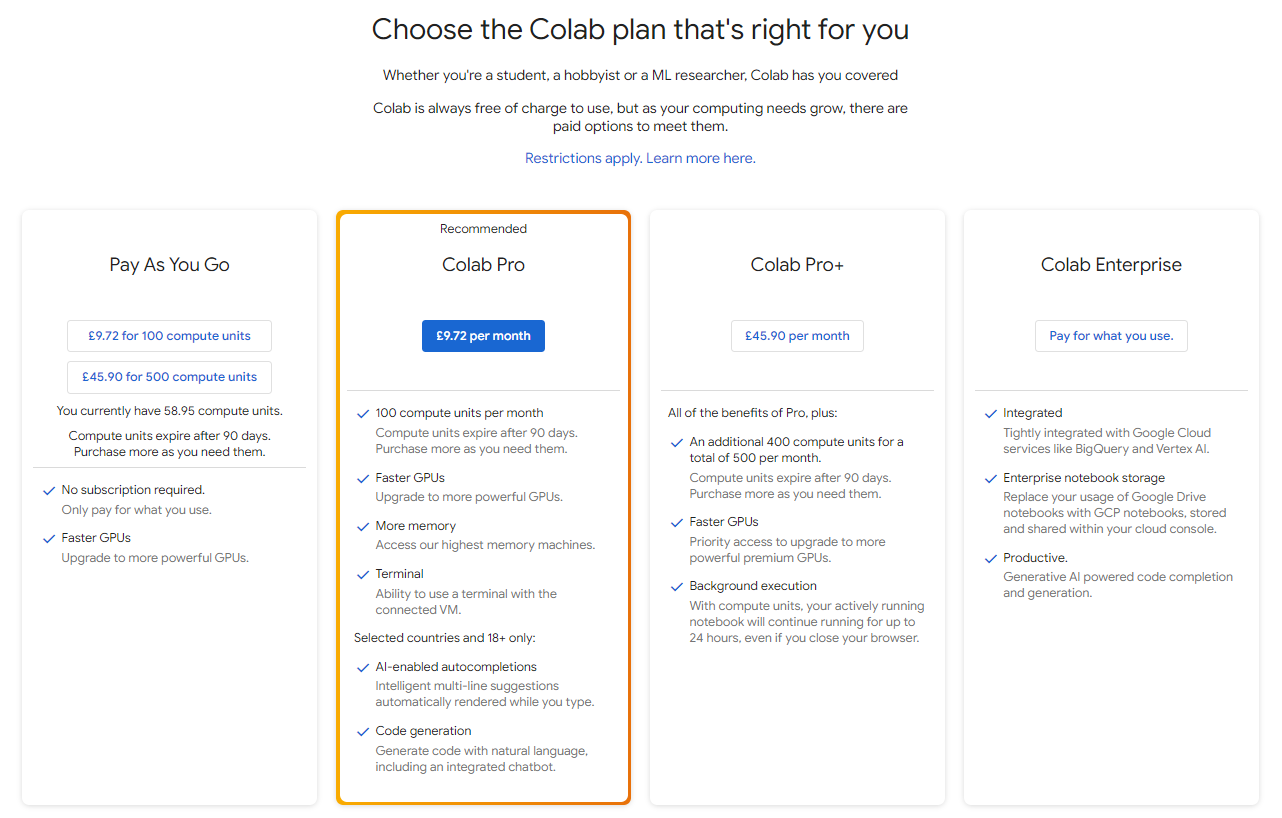
\includegraphics[width=0.7\textwidth]{Google Colab.png}
\caption[A screen-grab of the Google Colab subscription pricing as of March 2024.]{A screen-grab of the Google Colab subscription pricing as of March 2024. Image source: \url{https://colab.research.google.com/signup}.}
\label{fig:Google Colab}
\end{figure}
% -----------COULD REMOVE/CHANGE--------------
Despite its popularity, Google Colaboratory is not flawless. The biggest issue with this software is its steep pricing and quality at certain subscription levels. This section will analyse the question: are these levels worth the money?\\
As shown in Figure~\ref{fig:Google Colab}, there are four primary subscription levels. This analysis will not include ``Colab Enterprise" as this is typically used by larger bodies such as whole companies or research groups.\\
The free version of Colab, not shown in Figure~\ref{fig:Google Colab}, allows execution of small Python programs with a low power \acrshort{gpu}. One major problem with this level is that access to this acceleration is limited by an unspecified number of computation units. After you have used up your units, you are blocked from utilising this \acrshort{gpu} again. Furthermore, a lack of background execution makes this subscription level unstable, with cache eviction causing the webpage to lose the current runtime, along with potential training runs and results. Altogether, this makes the free level of Colab limited, unstable and not suitable for training large \acrshort{ml} models.\\
The ``Pay As You Go" level gives limited access to more powerful \acrshort{gpu}s. The amount of compute units given at this level is often used quickly, especially at the beginning of research when many different things are being trialled. Moreover, Google provides no recovery for interrupted runtimes, meaning that if credits run out halfway through a training run, results can be lost. This results in high money wastage.\\
The ``Colab Pro" level, kindly marked as recommended by Google, is an evil twin to the ``Pay As You Go" level. Although it provides similarly powerful \acrshort{gpu}s, more memory for running sessions and a terminal, it locks users into a subscription. The extra memory is a useful extension as notebooks can occasionally fill up RAM if too much data is loaded or variables are not cleared.\\
``Colab Pro" contains all the disadvantages of ``Pay As You Go" and the benefits are not significant enough to constitute entering into a subscription. Google does at least make it easy to cancel subscriptions\footnote{\url{https://colab.research.google.com/cancel-subscription}}.\\
I recommend utilising “Colab Pro+” as opposed to “Colab Pro”. This subscription level gives a huge 500 compute units, access to the fastest \acrshort{gpu} acceleration and background execution. The pricing of this level also saves at least £2.7 compared to ``Pay As You Go". Background execution saves money, time and effort by preventing runtimes from dying. However, this pricing is still very high, especially if this amount of credits is not required.\\
Overall, Google Colab is a double-edged sword; it is a useful tool, allowing fast development to those without access to hardware acceleration, however, it is an expensive option. Google Colab will not be used for this project due to the pricing and the alternative option of the \acrshort{csf}.\\
% My recommendataion, if Google Colab must be used, is to closely monitor compute unit amounts. ``Colab Pro+"``Colab Pro+" should be used due to its many benefits, downgrading to ``Pay As You Go" as project demand settles in its later stages.
\subsection{Computational Shared Facility}
% ------------COULD REMOVE THIS------------
The \acrfull{uom} \footnote{\url{https://www.manchester.ac.uk/}}, provides a high-performance computing cluster dubbed the \acrfull{csf} \footnote{\url{https://research-it.manchester.ac.uk/services/the-computational-shared-facility-csf/}}. This is provided for primarily staff and PhD students to carry out computationally intensive tasks or jobs requiring possibly hundreds of cores simultaneously.\\
The \acrshort{csf} is a free-to-use resource that staff and students can request access to. It is incredibly fast, consisting of thousands of CPU cores and 100 GPUs such as Nvidia\footnote{\url{https://www.nvidia.com/en-gb/}} V100 Volta and A100 Ampere GPUs.\\
Despite the various possible benefits, many students decide not to use the \acrshort{csf} due to its steep learning curve, batch job system and on-campus requirement.\\
\begin{figure}
\centering
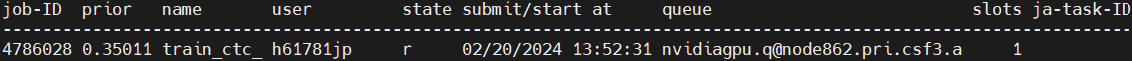
\includegraphics[width=0.9\textwidth]{CSF Example.png}
\caption[A screen-grab from MobaXTerm of a \acrshort{csf} job running.]{A screen-grab from MobaXTerm of a \acrshort{csf} job running. Here the \textit{qstat} command has been used to see the running jobs submitted from the current user. One job is running currently, titled ``train\_ctc\_based.txt".}
\label{fig:CSF Example}
\end{figure}
The \acrshort{csf} is a batch job system, requiring users to submit text files of requested commands and wait for the result. Figure~\ref{fig:CSF Example} shows an example of the job queue for the \acrshort{csf}. Below are listed some of the crucial commands for the \acrshort{csf}:
% ------------COULD REMOVE THIS------------
\begin{itemize}
  \item \textbf{qsub \textit{job\_script.txt}}: Submit a job file to be run
  \item \textbf{qstat}: See the list of jobs you have submitted. They can be listed as \textit{qw} (waiting in the job queue to run), \textit{r} (running) or \textit{Eqw} (Job has errored and will wait forever). If the job has already been completed then this command will show an empty queue
  \item \textbf{qdel \textit{id}}: Stop and delete the job with the ID specified
\end{itemize}
% ------------COULD REMOVE THIS------------
Some major hurdles encountered with the \acrshort{csf} during this project were:
\begin{itemize}
  \item Job files were prepared in Windows, causing an issue. Job files had to be prepared in a Linux format or converted using the \textit{dos2unix} command
  \item Running Juypter Notebook\footnote{\url{https://jupyter.org/}} files automatically required the use of the command \textit{jupyter nbconvert}
  \item Conda environments\footnote{\url{https://conda.io/projects/conda/en/latest/user-guide/tasks/manage-environments.html}} where required to install the correct versions of specific packages
  \item The correct and compatible versions of Cuda and TensorFlow\footnote{\url{https://www.tensorflow.org/install/source}} required installation within this environment
\end{itemize}
% ------------COULD REMOVE THIS------------
The code in Listing~\ref{lst: CSF Job} shows an example of a \acrshort{csf} job script. The script is used to automatically run Juypter notebooks for training.
\begin{lstlisting}[language=Bash, caption={[Example of a CSF job script]{Example of a CSF job script. Here the CSF Juypter module is loaded: this allows Juypter-based commands to be run. Then, the Conda environment is activated and the correct packages are installed and configured, based on debug information from the University. The notebook is then run before the environment is deactivated again.}}, label={lst: CSF Job}]
#!/bin/bash --login
#$ -cwd

#$ -l nvidia_a100=1
module load apps/binapps/jupyter-notebook/6.0.0 #Load Juypter module

source activate myenv #Activate Conda env

#Install correct Cuda and Tensorflow
conda install -y -c conda-forge cudatoolkit=11.8.0
pip install --isolated nvidia-cudnn-cu11==8.6.0.163 tensorflow==2.13.*
conda install -c nvidia cuda-nvcc --yes

#Configure based on information from UoM
CUDNN_PATH=$(dirname $(python -c "import nvidia.cudnn;print(nvidia.cudnn.__file__)"))
export LD_LIBRARY_PATH=$LD_LIBRARY_PATH:$CONDA_PREFIX/lib:$CUDNN_PATH/lib
export XLA_FLAGS=--xla_gpu_cuda_data_dir=$CONDA_PREFIX/lib

#Run the Juypter notebook experiment
jupyter nbconvert --execute --to notebook --ExecutePreprocessor.timeout=-1 --inplace proj_code/colabs/Train\ Video\ Based.ipynb

source deactivate
\end{lstlisting}
The \acrshort{csf} was utilised for this project. The \acrshort{csf} provides 4--5\,GB of RAM for free (with more requiring only a request) compared with Google Colab's 15 GB with more requiring a further subscription. The \acrshort{csf} does have a steep learning curve but it is reliable, scalable, efficient and free compared to Google Colab. The \acrshort{csf} provides the benefits of ``Colab Pro+" without the extreme pricing.\\
An SSH connection was required to access the \acrshort{csf} and submit jobs. However, due to a recent cyber incident, remote access to this network was suspended. Therefore all work was conducted on-campus via the MobaXterm\footnote{\url{https://mobaxterm.mobatek.net/}} application. This allowed for easy control over SHH connections.
\section{Data Generation Pipeline}
\label{sec: Data Generation Pipeline}
This section will outline the process used to generate useful data for training lip reading models and the source dataset selected for training. It will delve into the design decisions and processes employed for data preprocessing.\\
\begin{figure}
\centering
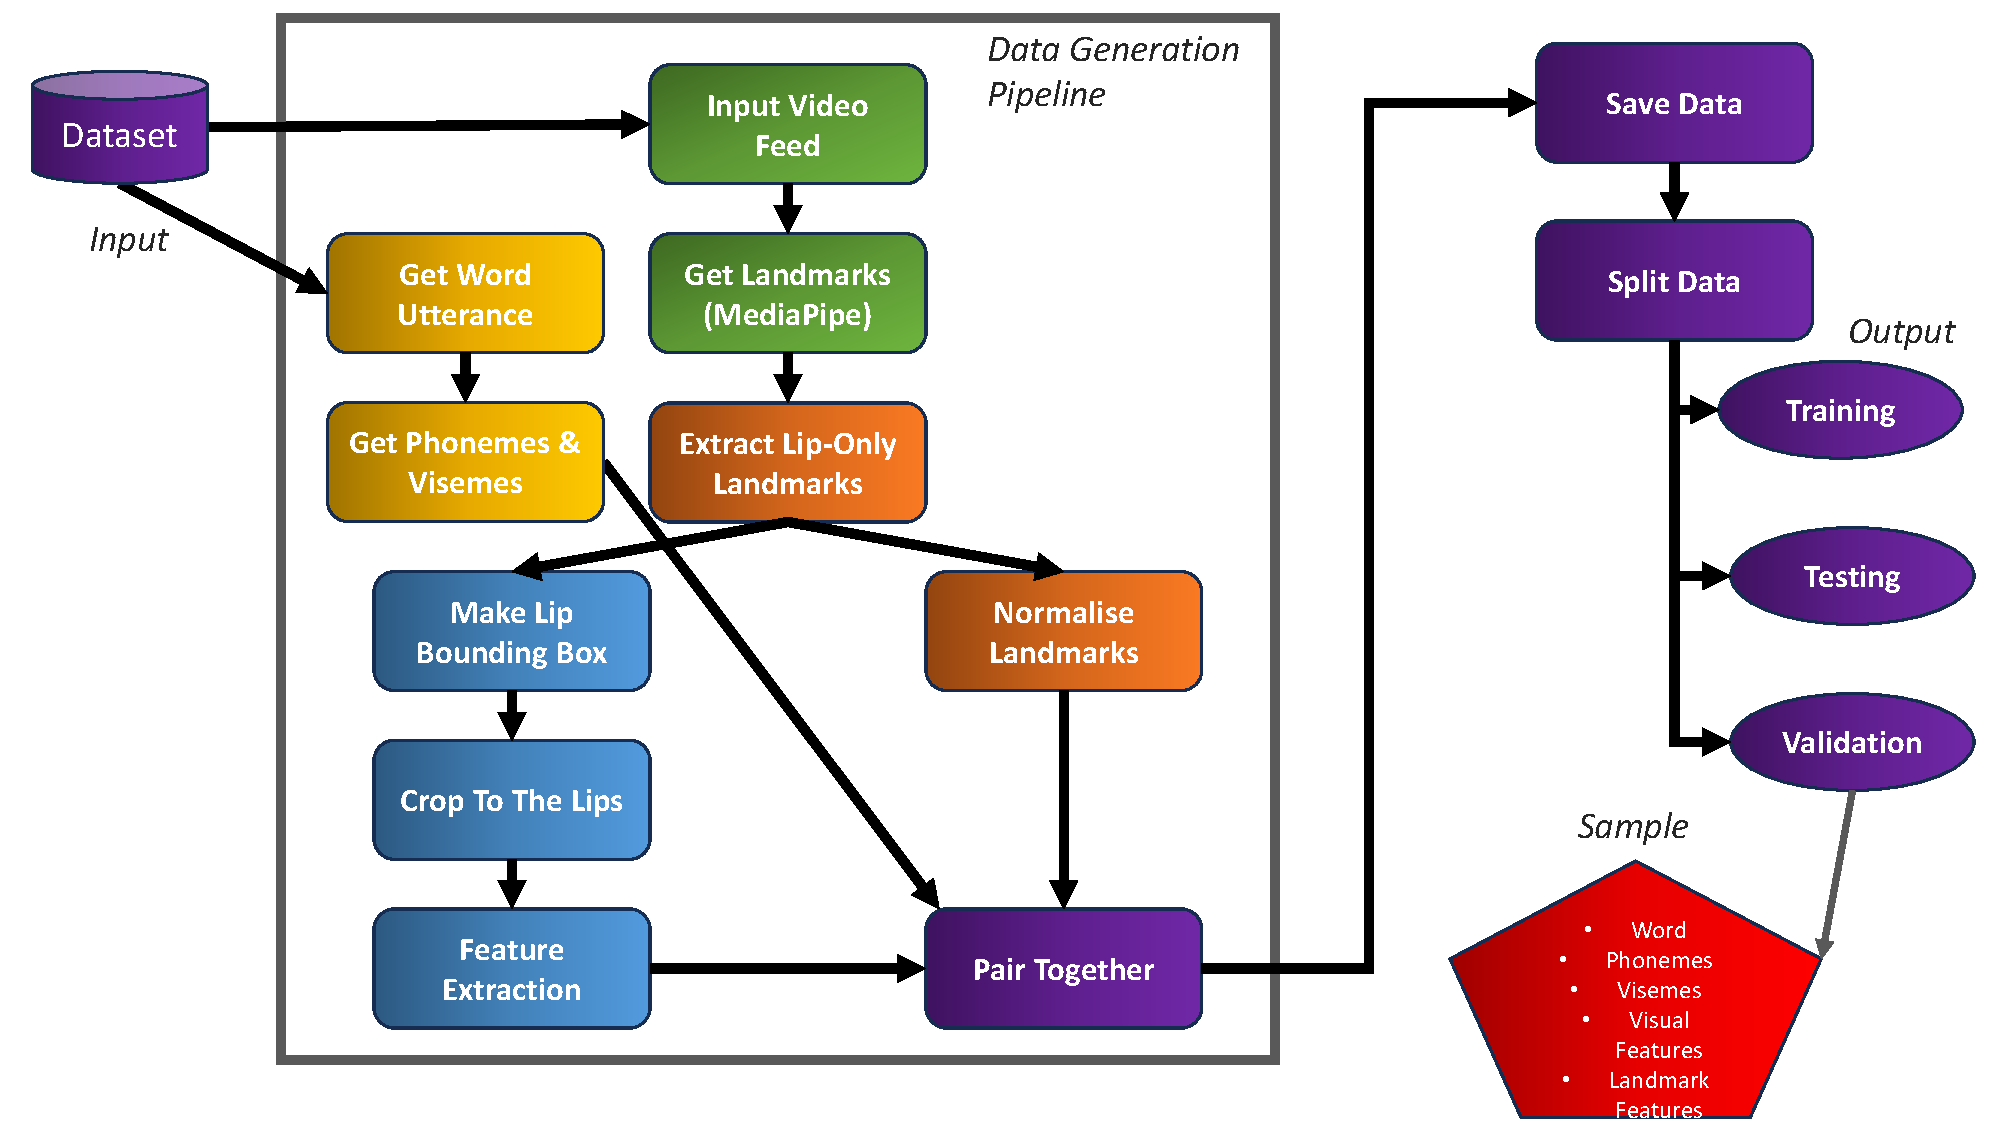
\includegraphics[width=1\textwidth]{Preprocessing Workflow.pdf}
\caption[The Data Generation Pipeline from the LRW data to split samples, ready for training.]{The Data Generation Pipeline from the LRW data to split samples, ready for training. This shows how data samples are constructed for training, combining the labels, visual features and landmark features. All data is preprocessed and saved before a data split is subsequently done.}
\label{fig:Data Gen Pipeline}
\end{figure}
The general process for data generation is shown in Figure~\ref{fig:Data Gen Pipeline}. MediaPipe was applied to each video from the dataset extracting facial landmarks which enabled a crop of the mouth to be taken. Feature extraction was done on the lip crops and the lip landmarks were normalised. This data was stored along with the word, \gls{phoneme} and \gls{viseme} utterances for the video. Data was split into three sets: training, testing and validation.\\
The overall data generation pipeline can be broken down into four primary stages:
\begin{enumerate}
    \item Landmark feature extraction, outlined in Section~\ref{sec: Landmark Feature Extraction}
    \item Visual feature extraction, outlined in Section~\ref{sec: Visual Feature Extraction}
    \item Word utterance processing, outlined in Section~\ref{sec: Word Utterance Processing}
    \item Random data splitting, outlined in Section~\ref{sec: Data Splitting} 
\end{enumerate}
\subsection{Dataset}
\label{sec: LRW Dataset}
For all of these experiments the same dataset and data split were maintained, ensuring consistent results and reliable comparison between the different models.\\
\begin{figure}
\centering
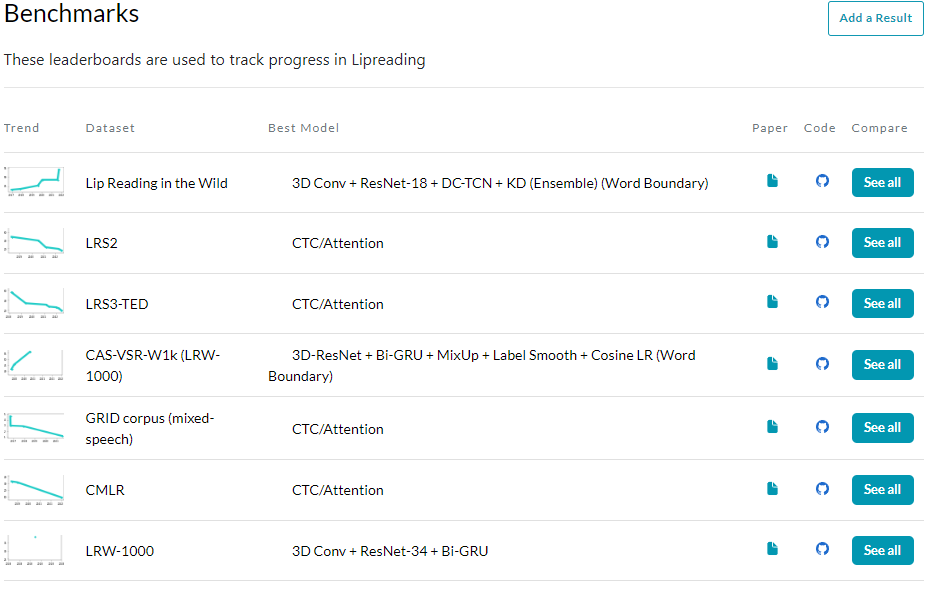
\includegraphics[width=0.7\textwidth]{Lipreading Benchmark.png}
\caption[The benchmark for lip reading via \acrshort{ml}]{The benchmark for lip reading via \acrshort{ml}. This shows some of the available datasets available for training lip reading models. Image source: \url{https://paperswithcode.com/task/lipreading}}
\label{fig:Lip Reading Benchmark}
\end{figure}
Shown in Figure~\ref{fig:Lip Reading Benchmark}, the choice of datasets was primarily between that of \gls{lrw}, \gls{lrs2}, \gls{lrs3}, \gls{lrw1000} and \gls{glips}. The final two of these were not considered because they are transcribed in alternative languages and therefore would pose an additional layer of complexity. Furthermore, \gls{lrs3} was not considered as the data is not available; the link\footnote{\url{https://www.robots.ox.ac.uk/~vgg/data/lip_reading/lrs3.html}} to this data leads to a 404 error.\\
The choice between \gls{lrw} and \gls{lrs2} depends primarily on the task being carried out. Both of these datasets are available upon request online\footnote{\url{https://www.robots.ox.ac.uk/~vgg/data/lip_reading/}}. \gls{lrw} was selected because its structure suits the task being carried out.\\
As shown in Figure~\ref{fig:LRW Structure}, \gls{lrw} consisted of a set of folders named after the primary word utterance within each video. As shown in Figure~\ref{fig:LRW Example 2}, each video consisted of 29 frames from BBC broadcasts. During these clips, a primary word was uttered, but possibly multiple other words were also spoken either before or after the primary utterance.\\
\begin{figure}
\centering
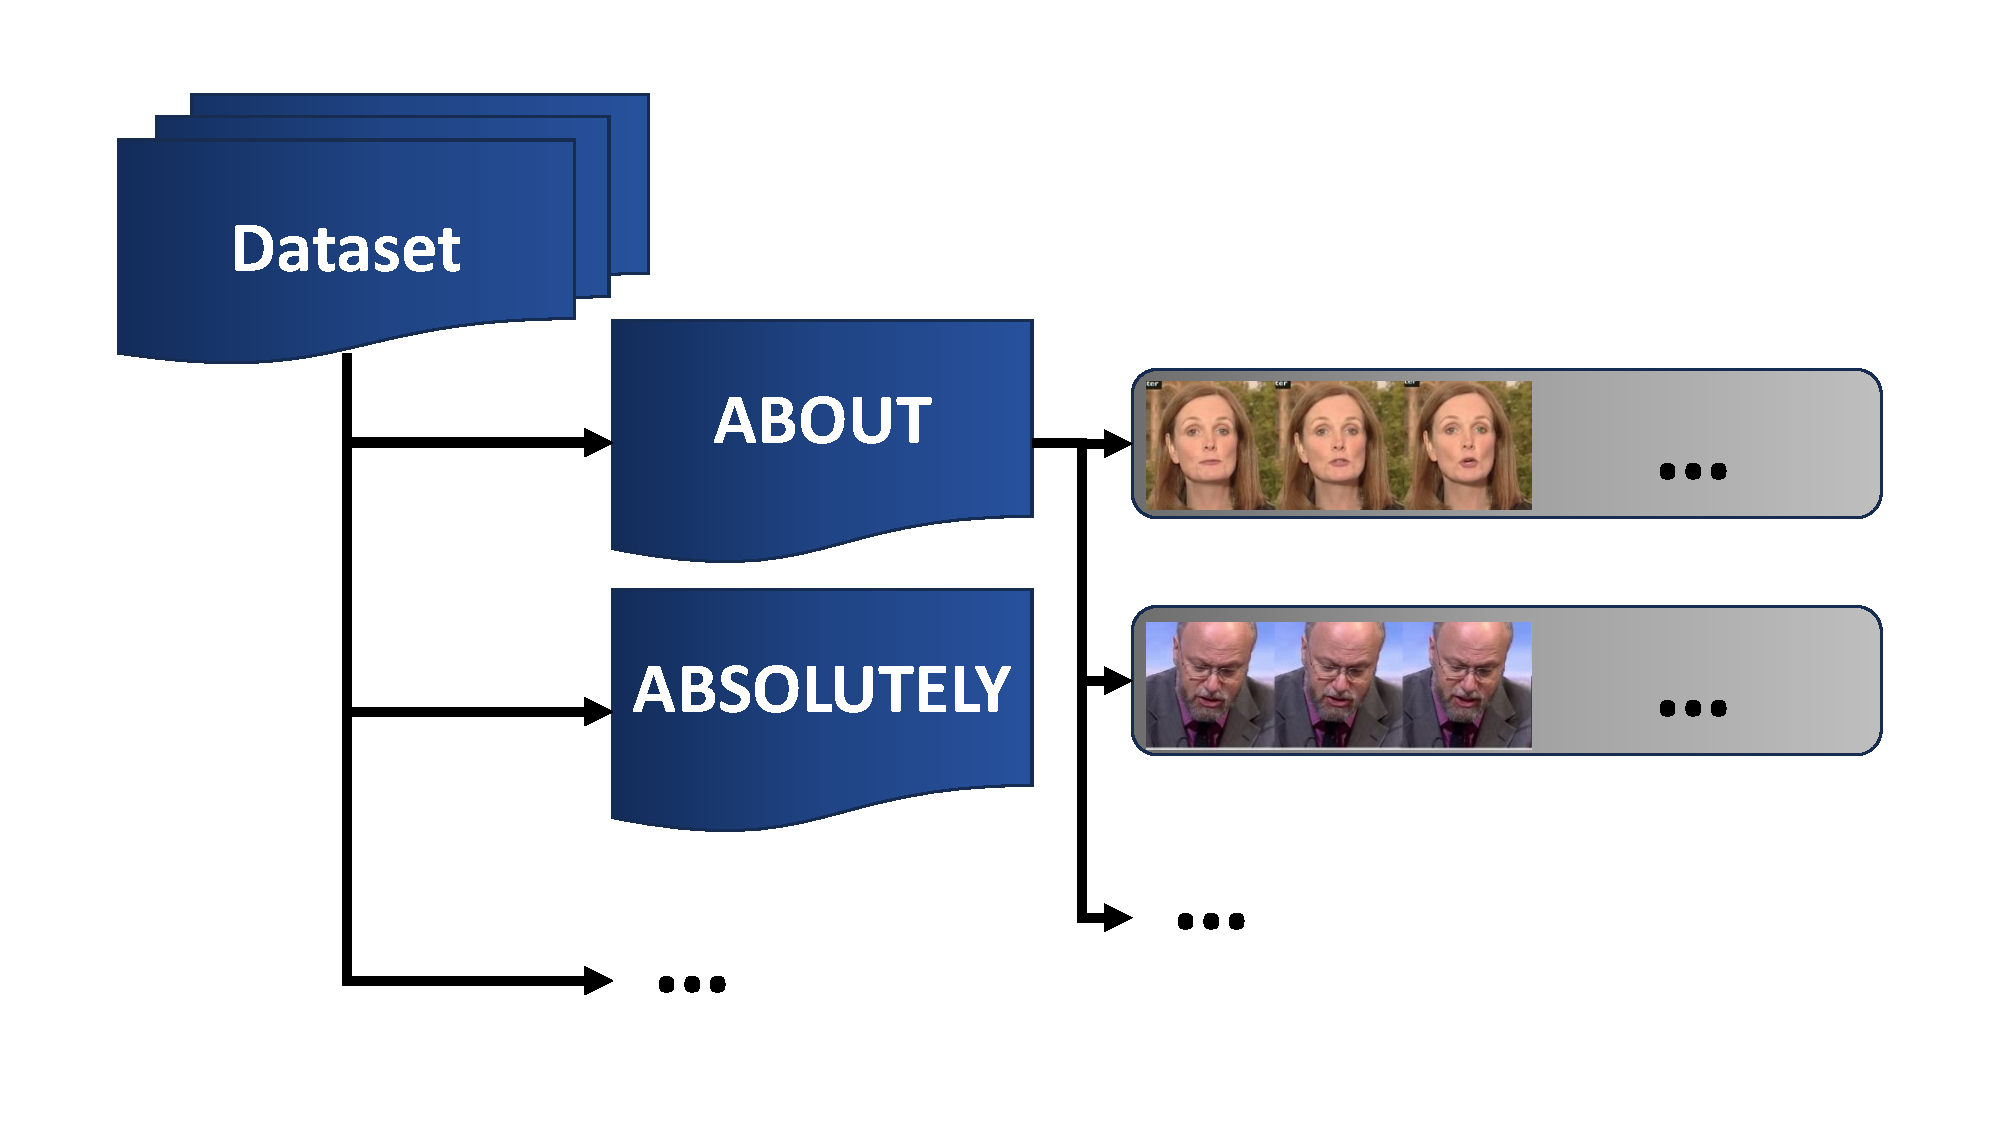
\includegraphics[width=0.7\textwidth]{LRW Structure.pdf}
\caption[The structure of the \gls{lrw} dataset.]{The structure of the \gls{lrw} dataset~\cite{Lip-Reading-In-The-Wild}. \gls{lrw} contains a set of directories labelled with the primary word being spoken. Each directory stores 1100 videos, each 29 frames long of BBC broadcasters saying a small set of words. The primary word spoken is within the middle of the video.}
\label{fig:LRW Structure}
\end{figure}
\begin{figure}
\centering
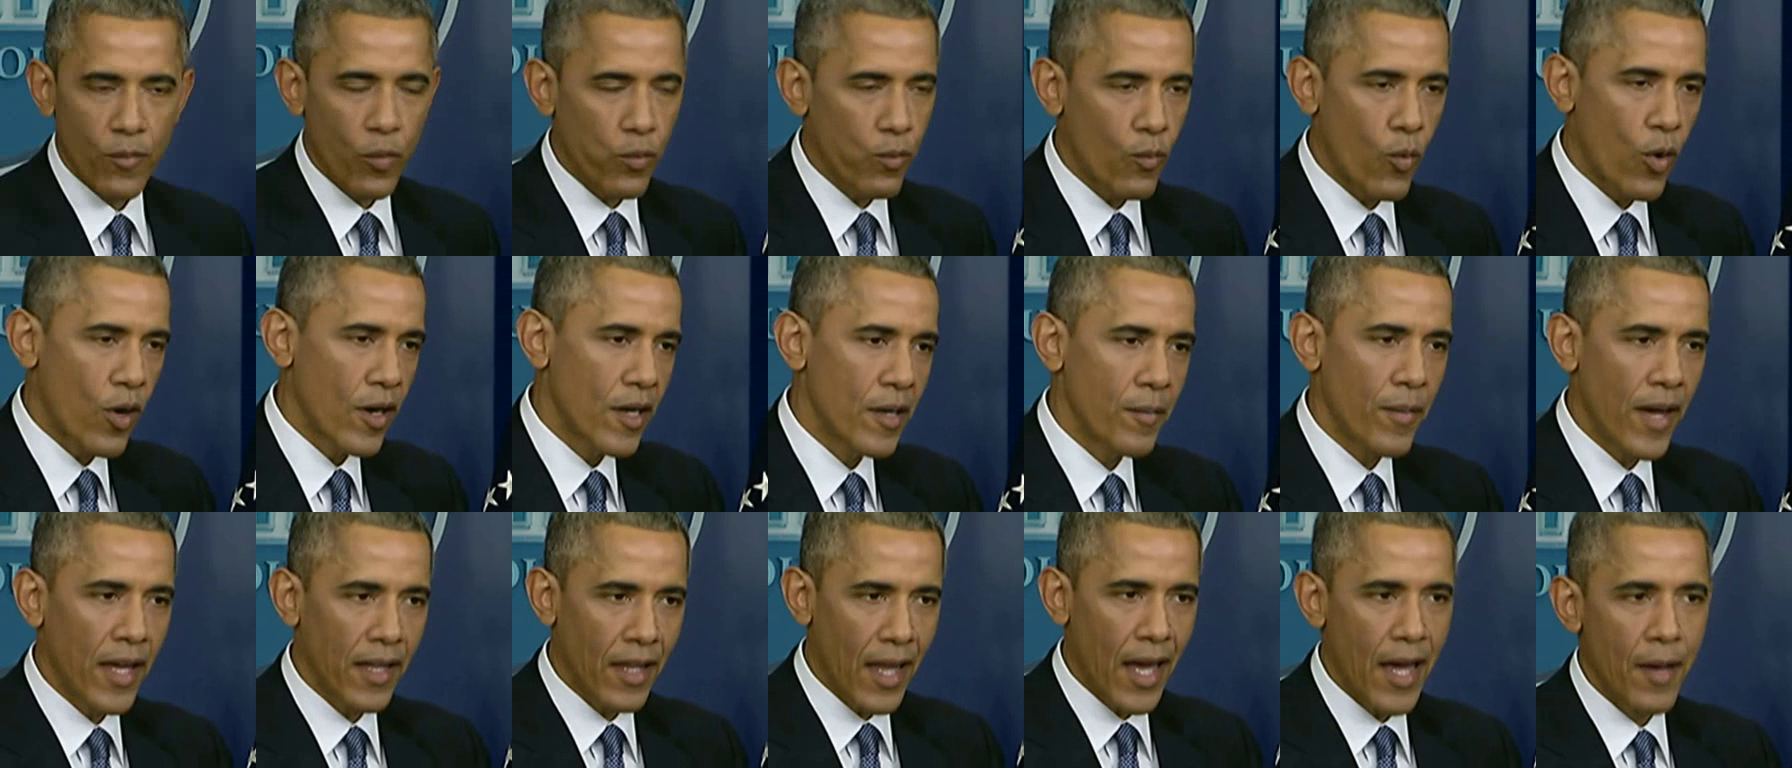
\includegraphics[width=0.7\textwidth]{LRW Example 2.png}
\caption[An extract from the \gls{lrw} dataset.]{An extract from the \gls{lrw} dataset~\cite{Lip-Reading-In-The-Wild}. This clip is labelled as ``ABOUT" but it contains the words ``worried about liability" with the final word half cut off.}
\label{fig:LRW Example 2}
\end{figure}
This structure benefits the model as it provides a large amount of data for each different word utterance, allowing training to fully understand the structure and intricacies of each word. Furthermore, the addition of extra, unlabelled words within clips adds variation to the data and produces models capable of recognising single words within sentences. This is similar to the original research carried out by Chung et al.~\cite{Lip-Reading-In-The-Wild}. The primary downside to \gls{lrw} is the possibility of \gls{overfitting} due to the extra noisy, word utterances.\\ 
The experiments involved training models capable of understanding a small subset of words. \gls{lrw} suited this better compared with \gls{lrs2} which has a collection of random videos, each with a sentence of labelled words. The diversity of words within \gls{lrs2} is useful but not for the task being carried out.\\
Four words were randomly selected for the models to be trained upon: \emph{about}, \emph{believe}, \emph{chance} and \emph{family}. These labels were transformed into \gls{one_hot_encoding}s for training. A subset of words was used to reduce training times and for model comparison. After preprocessing, 4,392 samples of these words were present within the dataset. This is slightly smaller than expected (4400) as MediaPipe could not find a valid face within some images, typically due to the orientation or clipping of faces within frames.\\
To gain access to the \acrshort{lrw} dataset, a request had to be sent to the BBC, explaining the work to be carried out. Once this request was approved, a login was provided for the \acrshort{lrw} website\footnote{\url{https://www.robots.ox.ac.uk/~vgg/data/lip_reading/lrw1.html}}, allowing data to be downloaded.\\
\gls{lrw} was split into seven parts, each approximately 10\,GB in size. Once downloaded, these parts then had to be concatenated together to form a zip file, containing the full dataset. To combine the file sections the command below was run
\begin{lstlisting}[language=Bash, caption={[Commands to combine the sections of the LRW dataset]{Commands to combine the sections of the LRW dataset. Note here that there are two separate sets of commands. The first are the commands presented on the LRW website however, this is seemingly for Linux. The second set is for Windows.}}, label={lst: Extract LRW}]
% Linux Commands:
cat lrw-v1* > lrw-v1.tar
tar -xvf lrw-v1.tar

% Windows Commands:
type lrw-v1* > lrw-v1.tar
\end{lstlisting}
At first these commands caused some issues. As the commands presented for the \acrshort{lrw} dataset are in Linux, and the development system utilised was Windows, some disparity was encountered. Running the commands above in Windows resulted in the file segments being repeatedly combined to form the zip file. After the set was concatenated once, the process was repeated seemingly infinitely.\\
Instead, a different command, shown in Figure~\ref{lst: Extract LRW}, had to be run before 7-Zip\footnote{\url{https://www.7-zip.org/}} was employed to extract these files.
\subsection{Data Preprocessing}
To prepare the data, the videos within \gls{lrw} directories specified as \emph{about}, \emph{believe}, \emph{chance} and \emph{family} were utilised. Each video within these directories was extracted and broken down into 29 individual frames. For each frame, MediaPipe was used to find landmark and visual features. The processes for these methods are detailed in the sections below. Some experiments involved just one of these data types whilst others used both.
\subsubsection{Landmark Feature Extraction}
\label{sec: Landmark Feature Extraction}
\begin{figure}
\centering
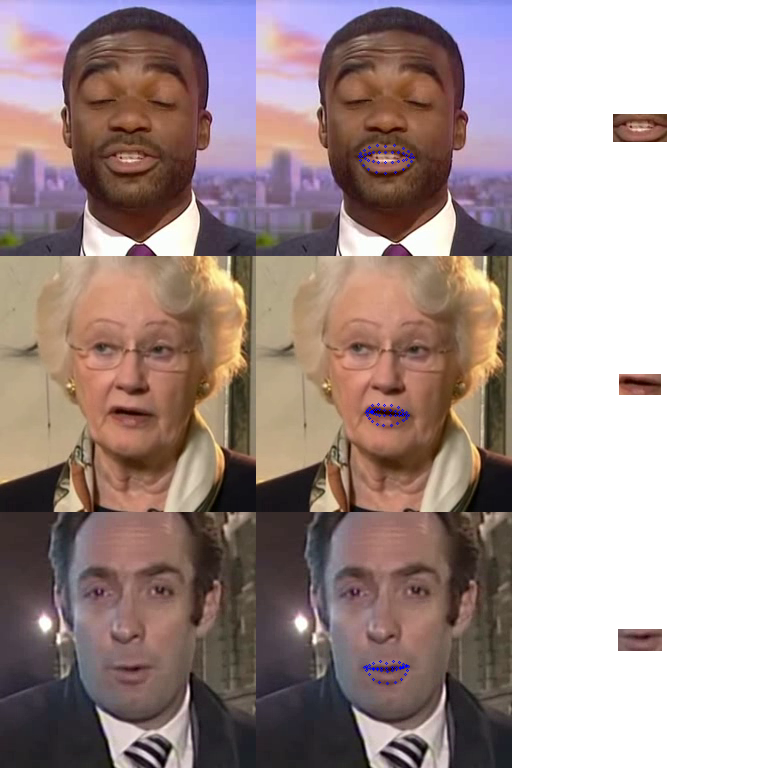
\includegraphics[width=0.7\textwidth]{MediaPipe Example.png}
\caption[An example of using MediaPipe to find the lip landmarks and lip region, from LRW data samples.]{An example of using MediaPipe to find the lip landmarks and lip region, from LRW data samples~\cite{Lip-Reading-In-The-Wild}. Here MediaPipe's Face Landmark Detection was used to generate facial landmarks which were then used to find and crop the lip region. The left images show the default image, the middle with lip-only landmarks highlighted and the right with the subsequent lip crop.}
\label{fig:MediaPipe Example}
\end{figure}
Explored in Section~\ref{sec:mediapipe}, MediaPipe provides a Face Landmark Detection\footnote{\url{https://mediapipe-studio.webapps.google.com/demo/face_landmarker}} model. This model was used to generate a set of 478 facial landmarks for each frame of the data subset used. Forty of these landmarks, specified in Listing~\ref{lst: MediaPipe Lip Indices}, corresponded to parts of the lips, so were extracted and used for training. Examples of this extraction process can be seen within Figure~\ref{fig:MediaPipe Example} and Figure~\ref{fig:Landmark Example}\\
\begin{figure}
\centering
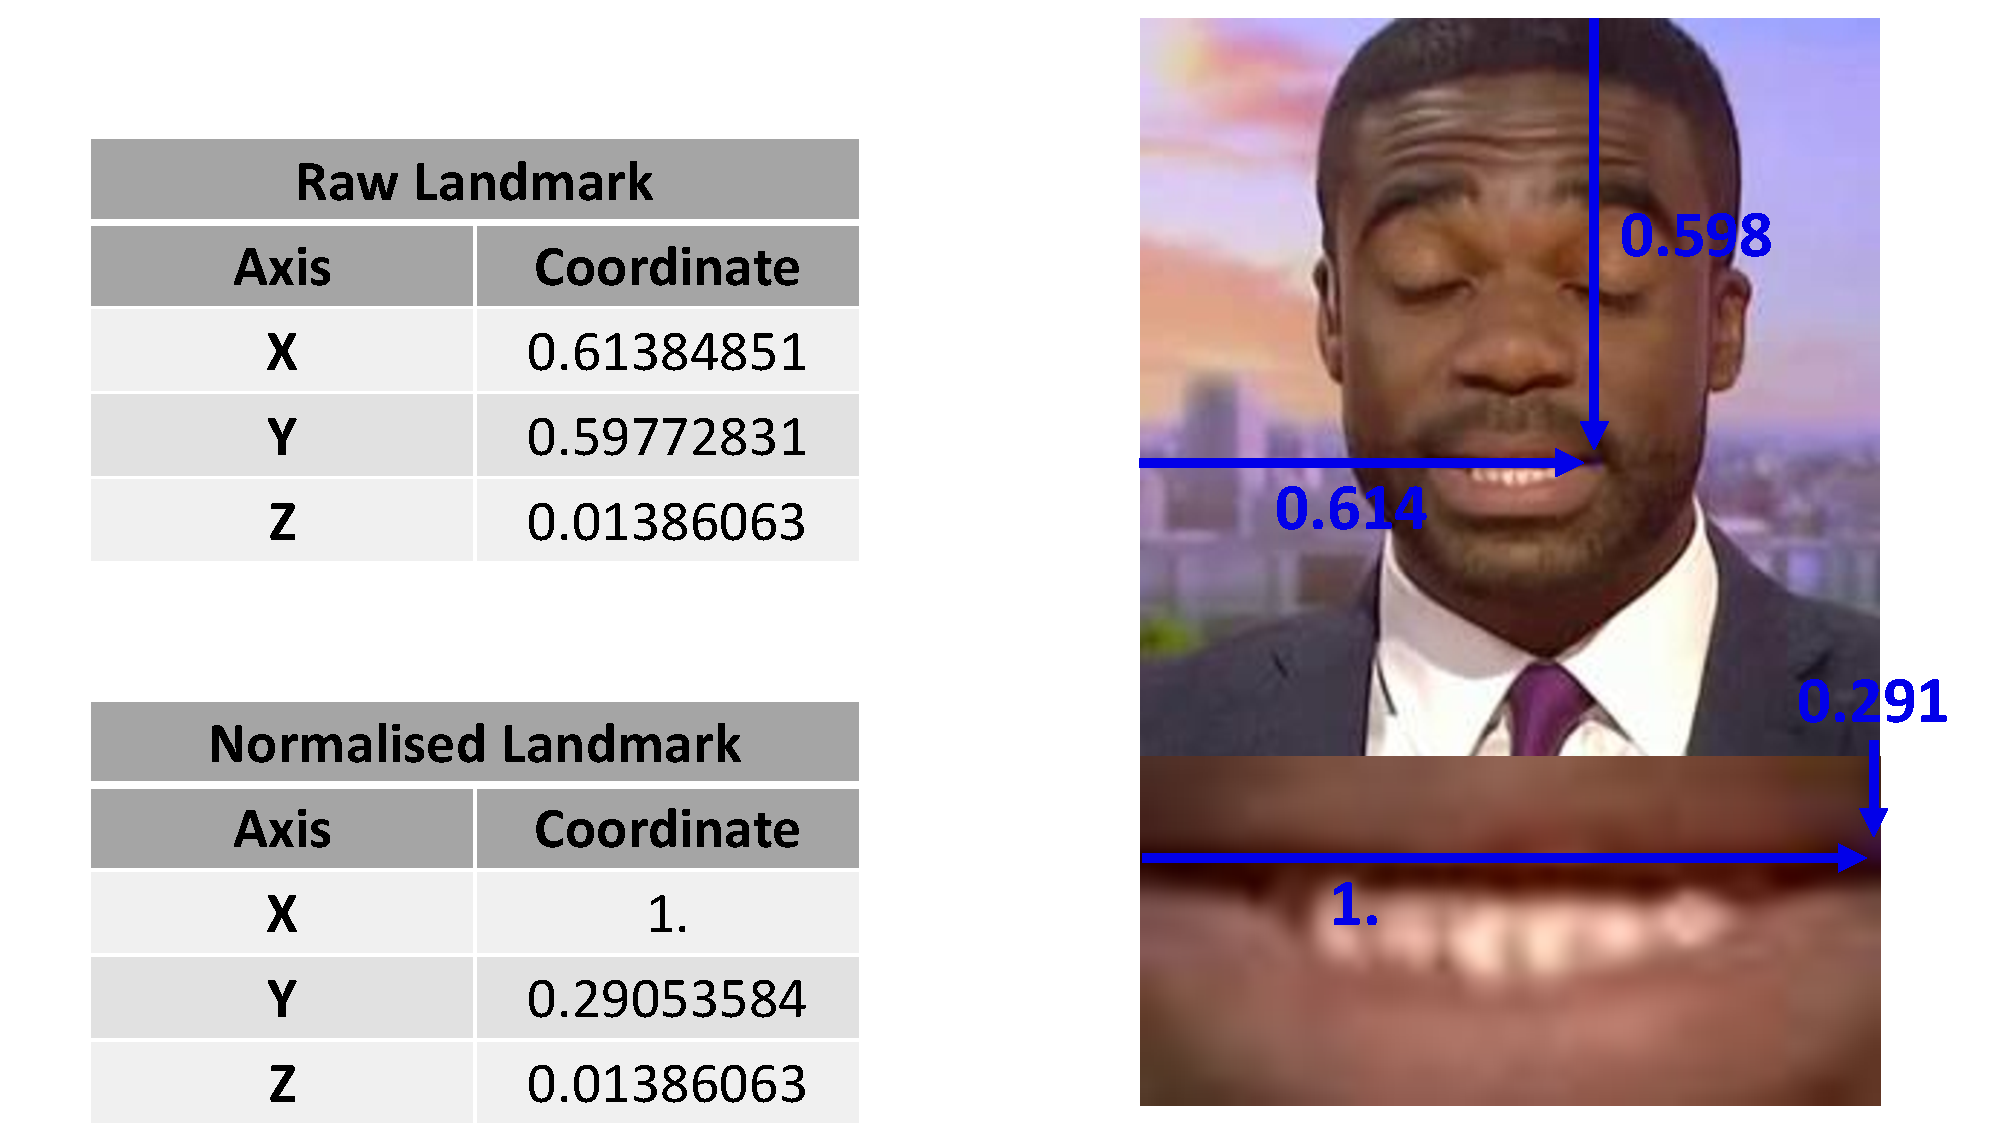
\includegraphics[width=0.7\textwidth]{Landmark Example.pdf}
\caption[An example of a normalised MediaPipe landmark]{An example of a normalised MediaPipe landmark, from the \gls{lrw} data samples~\cite{Lip-Reading-In-The-Wild}. Here MediaPipe is used to find facial landmarks. A single landmark is observed, which is displayed on the full image and the lip crop. The landmark is normalised based on the whole lip crop.}
\label{fig:Landmark Example}
\end{figure}
Landmarks are sets of $(X, Y, Z)$ coordinates relative to the position of facial landmarks within images. This is unsuitable for training as variation in the global position of faces within the video feeds can cause underfitting and make lip reading results incomparable. Therefore, normalisation was used to transform these coordinates into a proportionate form.\\
\begin{lstlisting}[language=Python, caption={[A list of the MediaPipe facial landmarks that correspond to the lips.]{A list of the MediaPipe facial landmarks that correspond to the lips. These correspond to the indices visualised within Figure~\ref{fig:mediapipe landmarks} as the facial landmarks associated with the lips.}}, label={lst: MediaPipe Lip Indices}]
lip_landmarks_outer_keys: typing.List[int] = [
    61, 185, 40, 39, 37, 0, 267, 269, 270, 409, 291, 375, 321, 405, 314, 17, 84, 181, 91, 146,
]
lip_landmarks_inner_keys: typing.List[int] = [
    78, 191, 80, 81, 82, 13, 312, 311, 310, 415, 308, 324, 318, 402, 317, 14, 87, 178, 88 95,
]
\end{lstlisting}
The mathematical function for this normalisation is shown below
\[X_i = \frac{X_i - X_l}{w},\]
\[Y_i = \frac{Y_i - Y_l}{h},\]
\[Z = Z,\]
where $(X_l, Y_l, 0)$ corresponds to the upper left coordinate of a bounding box created using all of the lip landmarks (defined in Section~\ref{sec: Visual Feature Extraction}), $(X_i, Y_i, 0)$ correspond to the coordinates of the $i$th lip landmark, and $w$ and $h$ are the width and height respectively of the lip bounding box in the image.\\
The width, $w$, and height, $h$, of the lip bounding boxes were formulated using the equations below
\[w = \max\{X_1, X_2,...X_{40}\} - \min\{X_1, X_2,...X_{40}\},\]
\[h = \max\{Y_1, Y_2,...Y_{40}\} - \min\{Y_1, Y_2,...Y_{40}\}.\]
The $Z$ coordinate was not normalised as this represents the depth of a landmark within an image. Thus, it is less useful for training and not relative to the image coordinates.\\
Once the landmarks were normalised they were saved to the preprocessed dataset.
\subsubsection{Visual Feature Extraction}
\label{sec: Visual Feature Extraction}
Landmark features are not enough on their own. There is substantial, relevant data related to speech that is not captured by the placement of the lips alone. For example, the teeth and tongue are both key to distinguishing certain \gls{phoneme}s yet not captured by MediaPipe. Utilising wider visual features is a technique adopted by various other successful lip reading systems~\cite{Lip-reading-techniques} and has been proven to produce better results~\cite{lipreading_with_attention}.\\
To produce visual features, the lip landmarks extracted in the previous stage were reused to create a bounding box around the lips. This bounding box was used to take a crop of each frame of the videos from \gls{lrw}.\\
To find the bounding box, defined by the coordinates $(X_l, Y_l)$ (for the top left corner) and $(X_r, Y_r)$ (for the bottom right corner), the following calculations were carried out:
\[X_l = \min(X_1, X_2,...X_{40})\]
\[Y_l = \min(Y_1, Y_2,...Y_{40})\]
\[X_r = \max(X_1, X_2,...X_{40})\]
\[Y_r = \max(Y_1, Y_2,...Y_{40})\]
Where $X_i$ defines the $X$ coordinate of lip landmark $i$ and $Y_i$ defines the $Y$ coordinate of lip landmark $i$.\\
InceptionV3 Imagenet \footnote{\url{https://keras.io/api/applications/inceptionv3/}}~\cite{InceptionV3} was used for visual \gls{feature_extraction} of the lip crops.\\
InceptionV3 Imagenet is lightweight and has high performance, making it useful for devices that might not use a GPU, whilst still boasting very high accuracy~\cite{InceptionV3}. It has a straightforward implementation via Keras. Possible future work could aim at experimenting with alternative feature extractors to compare performance metrics.\\
As shown in Figure~\ref{fig:Visual Feature Extraction}, lip crops were passed through the InceptionV3 Imagenet feature extractor, generating 2048 long feature vectors. Visual features were paired with the corresponding landmark features before being saved.
\begin{figure}
\centering
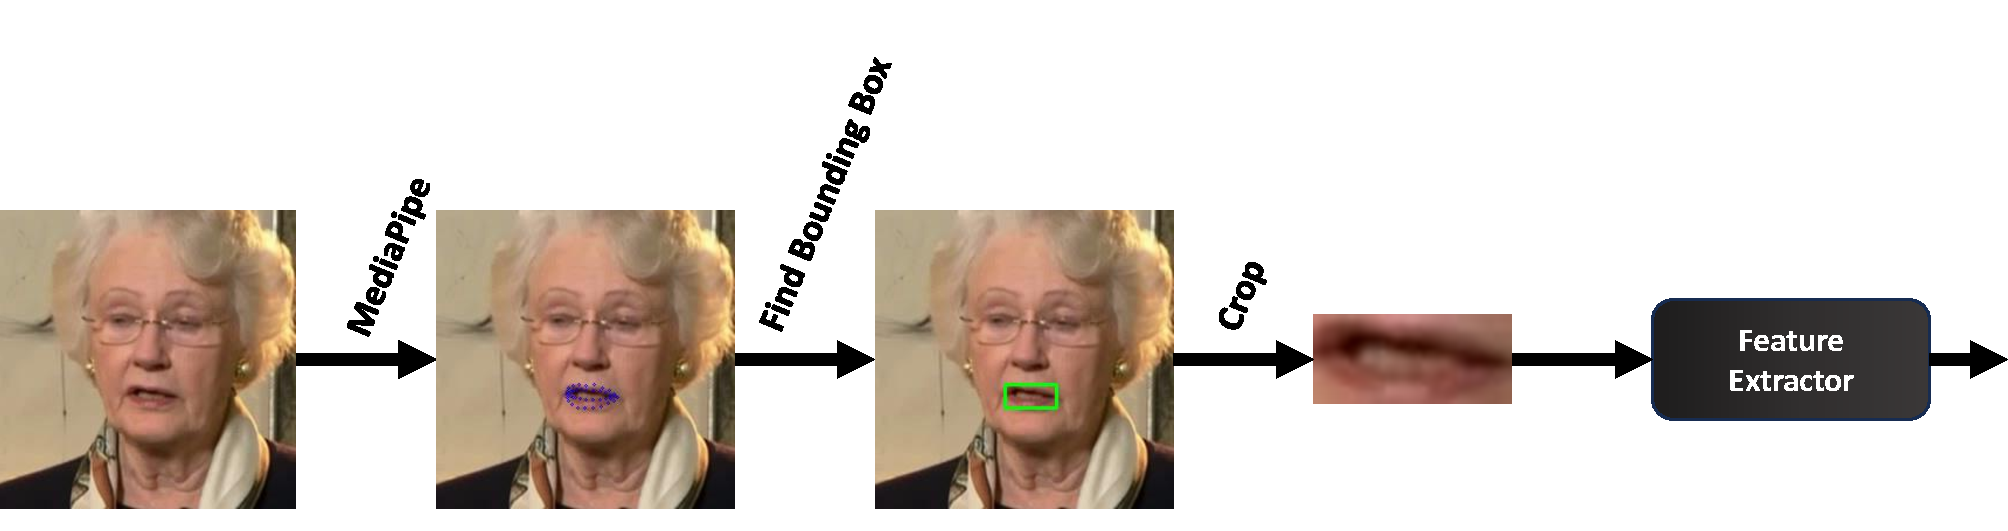
\includegraphics[width=0.7\textwidth]{Visual Feature Extraction.pdf}
\caption[The process of visual feature extraction.]{The process of visual feature extraction. MediaPipe is used to find lip landmarks. A bounding box is made surrounding all landmarks before a crop is taken. The crop is passed into a feature extractor.}
\label{fig:Visual Feature Extraction}
\end{figure}
\subsection{Word Utterance Processing}
\label{sec: Word Utterance Processing}
During training, videos were classified into a set of different classes:
\begin{itemize}
    \item The \textbf{words} spoken: \gls{multi-class} and \gls{single-label}
    \item The \textbf{letters} of words spoken: \gls{multi-class} and \gls{multi-label}
    \item The \textbf{\gls{phoneme}s} uttered: \gls{multi-class} and \gls{multi-label}
    \item The \textbf{\gls{viseme}}s expressed: \gls{multi-class} and \gls{multi-label}
\end{itemize}
\Gls{lrw} is currently annotated with only the words (and, therefore, also the letters) spoken within videos. Thus, both the \gls{phoneme}s and \gls{viseme}s for these had to be generated automatically.\\
To produce the \gls{phoneme}s, from words, the Python library NLTK\footnote{\url{https://www.nltk.org/_modules/nltk/corpus/reader/cmudict.html}} was used. Described in Section~\ref{sec: nltk}, this library can be used to convert words into their constituent \gls{phoneme}s via the Carnegie Mellon Pronouncing Dictionary (cmudict).\\
\begin{figure}
\centering
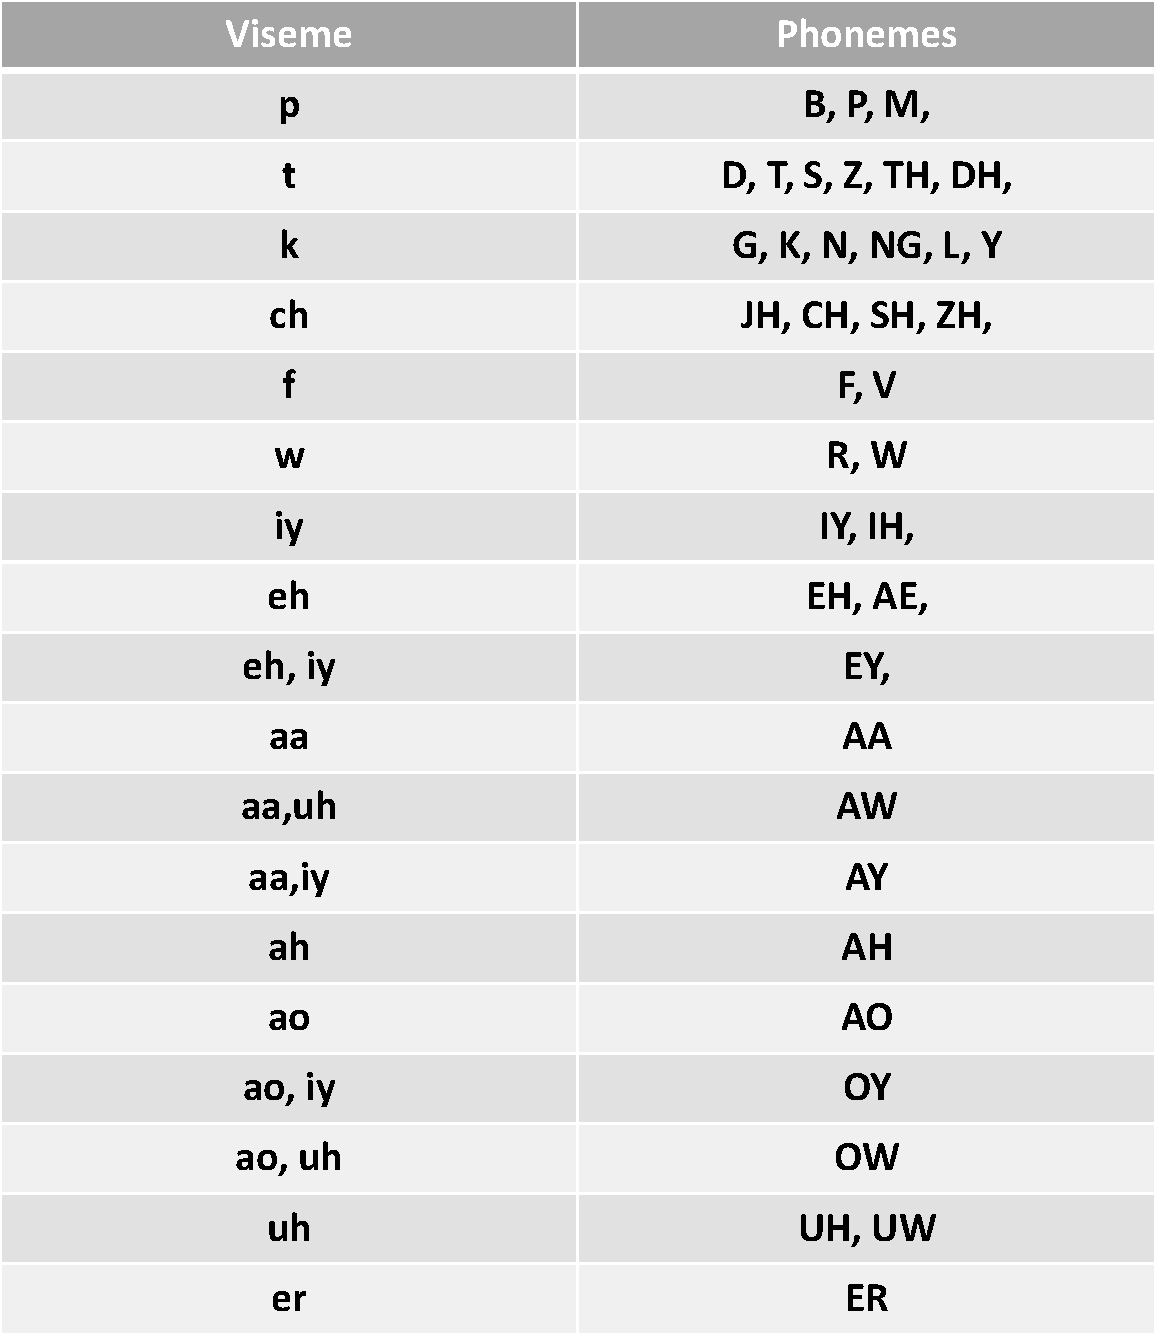
\includegraphics[width=0.7\textwidth]{P2V Mapping.pdf}
\caption[The adopted \acrshort{p2v} mapping, as proposed by Lee et al. and promoted by Bear et al.]{The adopted \acrshort{p2v} mapping, as proposed by Lee et al.~\cite{best_phoneme_viseme_mapping} and promoted by Bear et al.~\cite{phoneme_viseme_mapping_review}. This shows which \gls{phoneme}s fall into each \gls{viseme} group. Some \gls{phoneme}s are made up of multiple \gls{viseme}s and are therefore marked as such. There are thirteen \gls{viseme}s in total (and an additional blank \gls{viseme}, although this has not been added above).}
\label{fig:P2V Mapping}
\end{figure}
As explained more in Section~\ref{sec: Lip Reading}, retrieving the \gls{viseme}s of words is a harder task. Classification based on \gls{viseme}s is potentially a more fruitful endeavour for classification; \gls{viseme}s relating more closely to the visual aspects of language compared with letters or \gls{phoneme}s. However, there currently exists no defined \gls{viseme} set, let alone a tool for \acrfull{p2v} conversion.\\
For this set of experiments, as suggested by Bear et al.~\cite{phoneme_viseme_mapping_review}, the \acrshort{p2v} mapping proposed by Lee et al.~\cite{best_phoneme_viseme_mapping} was employed for \acrshort{p2v} conversion. This is shown within Figure~\ref{fig:P2V Mapping}. Note that some of the \gls{phoneme}s have two overlapping \gls{viseme}s (such as ``EY" and ``AW"). Although Lee et al.~\cite{best_phoneme_viseme_mapping} do not elaborate upon this, the reason for this is likely that some \gls{phoneme}s required multiple \gls{viseme}s to express.\\
\Gls{phoneme}s were converted into \gls{viseme}s using a Python dictionary. Once words had equivalent phonetic and visual forms, these data labels were exported with the corresponding data samples.
\subsection{Data Splitting}
\label{sec: Data Splitting}
\begin{figure}
\centering
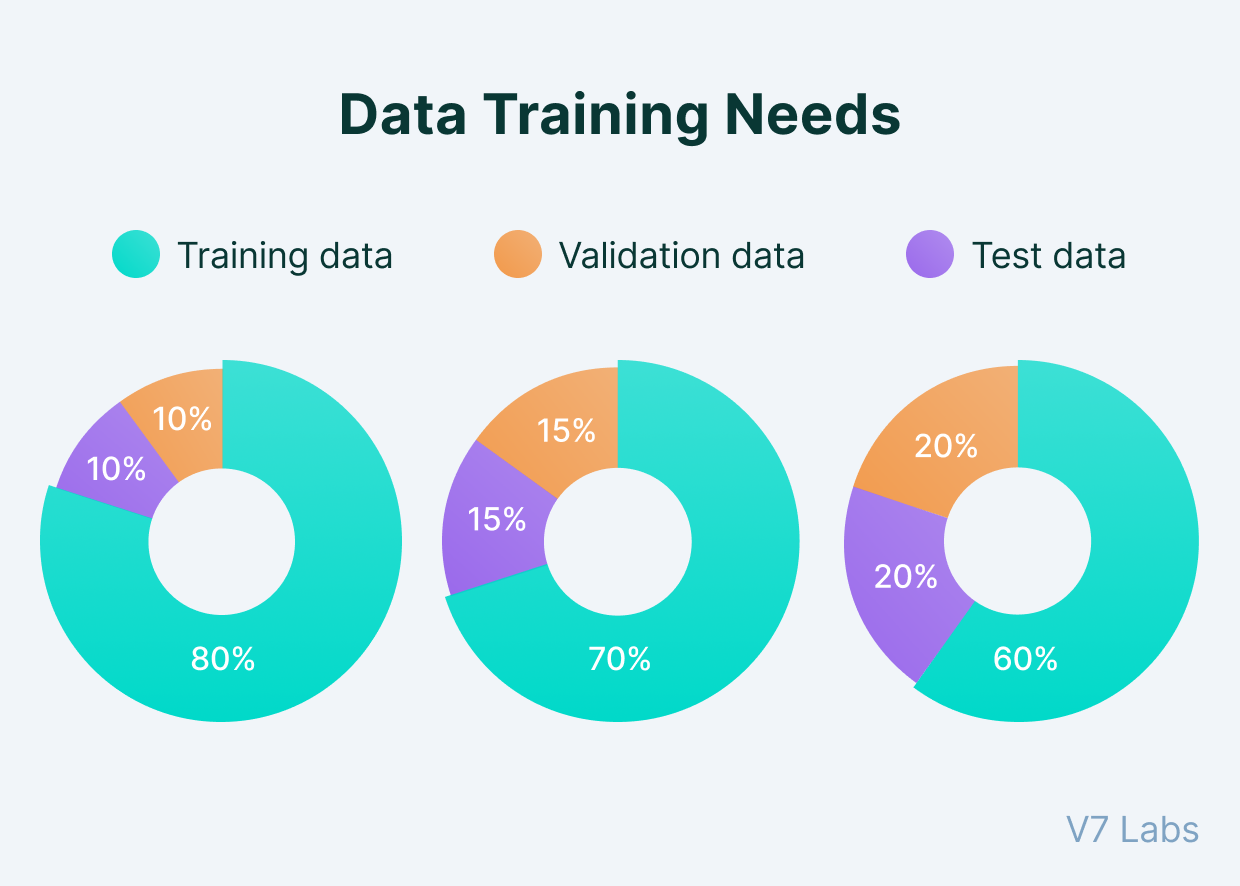
\includegraphics[width=0.5\textwidth]{Data Split Diagram.png}
\caption[A diagram of some common data split ratios used in \acrfull{ml}.]{A diagram of common data split ratios used in \acrfull{ml}.}
\label{fig:Data Split}
\end{figure}
Data splitting refers to the process of separating data into multiple sets, one to train the \acrshort{ann} and another to evaluate it~\cite{Data-Splitting_2}.\\
There are three typical sets for data splitting: training, testing and validation. The training set is used to train and optimise the model's parameters. The validation and testing sets are used to provide an unbiased view of the model's performance, kept separate to prevent \gls{overfitting}. The validation set is used to evaluate the model's performance and fine-tune its hyperparameters throughout training. The testing set is used to evaluate the model's final, overall performance and to directly compare different models.\\
There are various methods of data splitting, including but not limited to \acrfull{srs}, trial-and-error and systematic sampling~\cite{Data-Splitting}. These methods for data splitting primarily affect the variance of the model error. For example, trial-and-error sampling estimates the model error with lower variance than other methods~\cite{Data-Splitting}. For this research, the simple and easy-to-implement \acrshort{srs} was utilised during training, testing and validation even despite its high variance.\\
As shown in Figure~\ref{fig:Data Split}, there are different proportions of data split. Here data was split by randomly shuffling the data samples and selecting the first 80\% of samples for training, the next 10\% for testing and the final 10\% for validation. This is a common data split used within \acrshort{ml} projects.
\section{Design of Experiments}
This section will cover the structure of experiments covered within this research, including the many different design decisions and principles followed.
\subsection{Experiment Structure}
\begin{figure}
\centering
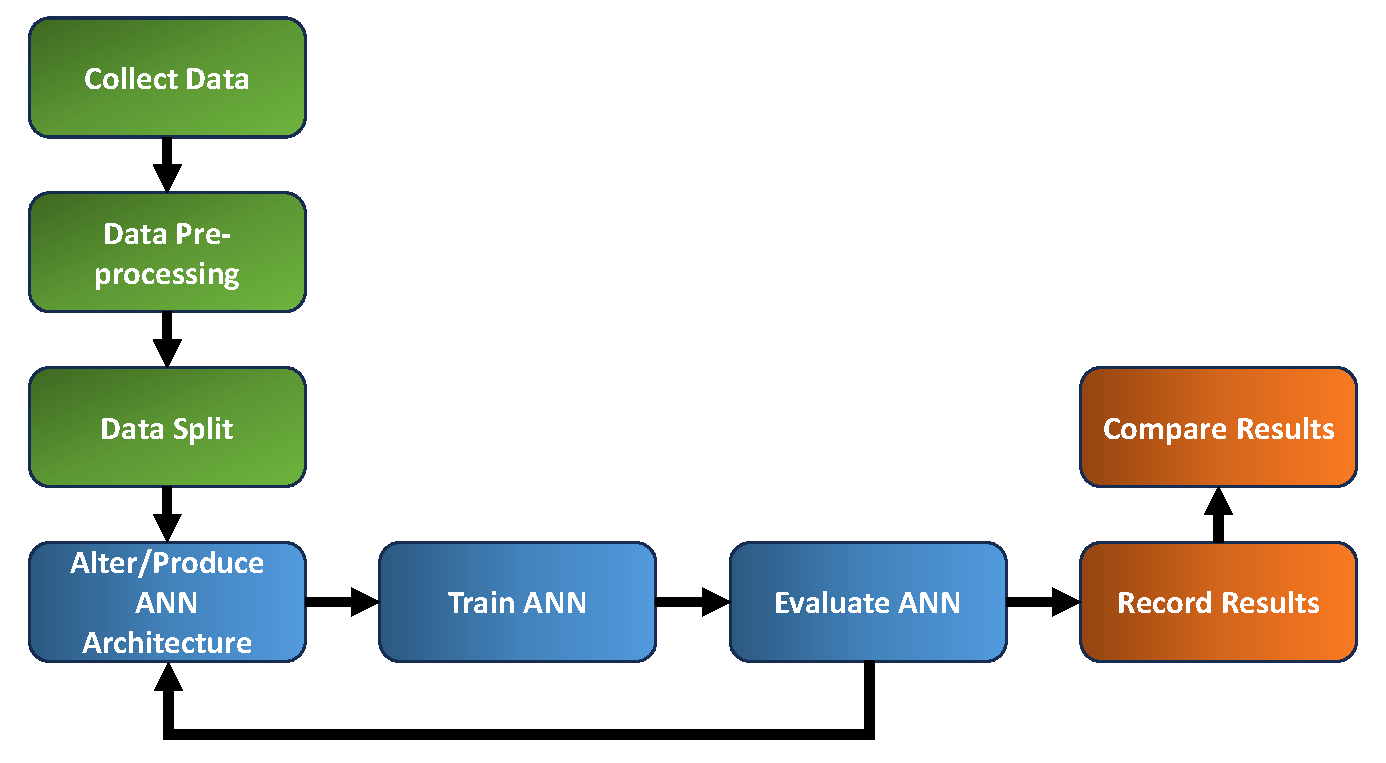
\includegraphics[width=0.7\textwidth]{Experiment Workflow.pdf}
\caption[The workflow adopted within the experiments.]{The workflow adopted within the experiments. The green section shows the steps that were carried out first and only once. The blue section was repeated several times, for each experiment. This section shows the iterative nature of the experiments, where changes are repeatedly made to gather further results. The orange section shows the critical reflection within this research.}
\label{fig:experiment workflow}
\end{figure}
The experiment structure is a key design decision that will inform the reliability of results and help to better compare alternative lip reading architectures. This structure is depicted in Figure~\ref{fig:experiment workflow}.\\
After data was collated and preprocessed, a set of experiments were carried out. The \acrshort{ann} was repeatedly altered, trained and evaluated to study the impact that various hyperparameters had on lip reading.\\
Models were trained using the training and validation sets, employing early stopping as specified within Section~\ref{sec: Early Stopping}. For each experiment, the optimal models were loaded back in and run against the testing dataset. This was used to objectively capture the performance on unseen data. The accuracy, loss and \acrfull{wer} (as defined in Section~\ref{sec: JiWER}) were observed.\\
Models were compared via their validation and testing metrics to find the best hyperparameter settings and draw conclusions as to the difficulties or benefits of different methods.\\
% Eg. Varying only 1 thing at a time. Finding the accuracy, loss & comparing them.
There were three principles fostered for these experiments:
\begin{itemize}
    \item Maintain the data split
    \item Make single changes between experiments --- changes can be large or small
    \item Maintain optimal changes to produce increasingly optimal models
\end{itemize}
The first concern is that of data. To allow for better model comparison, the same data sets should be employed to train and then evaluate the different models. This makes them directly comparable. Therefore, the data split algorithm was incorporated into the data generation pipeline, maintaining the split between the different experiments. This had the benefit of saving computation and processing by avoiding repeated, redundant data splits. The data split was made on each word class individually rather than the entire dataset. This ensured similar quantities of each data class for training, testing and validation.\\
The next concern is how to compare different experiments. Typically, only one thing should be varied between experiments to ensure that any changes in performance can be attributed directly to the change made. This is a hard task for \acrshort{ml}, where many different parameters are at play. Furthermore, this is made difficult by the definition of what a ``single change" entails: is this a single parameter change or a whole different \acrshort{ann} architecture? Early stopping, explained further in Section~\ref{sec: Early Stopping}, means that models could be trained for varying numbers of epochs which adds further variation. For this research, only one thing was purposefully altered, for example batch size or \acrfull{lr}. Changes between experiments could be more extensive, such as trying a whole different model architecture, but these changes were fully documented for this reason. Variation due to early stopping could not be avoided compared with the potential benefit this method poses to the performance of models.\\
The final principle is maintaining optimal changes to models where possible. When beneficial changes were discovered, these were maintained between experiments. This ensured an increasing performance throughout.
\subsection{Early Stopping}
\label{sec: Early Stopping}
For all training runs, early stopping was employed to save the best model weights. This was achieved using Keras's callback, ModelCheckpoint\footnote{\url{https://keras.io/api/callbacks/model_checkpoint/}}. This was configured to monitor the validation loss and save the model with the best performance. This would ensure the model is saved before \gls{overfitting} occurs and metrics worsen.
\subsection{Learning Rate}
\label{sec: Learning Rate}
The Adam optimiser was used in conjunction with exponential decay during training. Exponential decay was utilised to decay the \acrshort{lr} over time, as the local minimum was approached, thus scaling Adam's effect over time.\\
Adam, or adaptive moment estimation optimiser, is a modern \acrshort{lr} scheduler made popular due to its effectiveness, simplicity and handling of large amounts of data~\cite{Adam_OG}. In addition, Keras provides an easy-to-use Adam optimiser\footnote{\url{https://keras.io/api/optimizers/adam/}}. Adam works by selectively adjusting the \acrshort{lr} for each parameter, based on the history of that parameter~\cite{Adam_OG}.\\
Exponential decay is a method of lowering \acrshort{lr} over time, based on the current epoch. The benefit of using a decay is that a higher initial \acrshort{lr} can be employed at first, preventing \acrshort{ann}s from learning noisy data. The \acrshort{lr} is then reduced throughout, as the model converges to a global minimum in the loss. This reduces the negative impact on model performance during the early stages of training~\cite{benefit_of_decay}. Exponential decay is a popular and simple method of this, as defined below
\[lr_{new} = lr_{initial} \cdot e^{-D \cdot n},\]\\
where $lr_{new}$ is the updated \acrshort{lr} for the current epoch $n$, $lr_{initial}$ is the initial \acrshort{lr} and $D$ is the decay rate. The decay rate is a further parameter introduced with exponential \acrshort{lr} decay, used to control the rate of change.\\
In Keras, exponential decay\footnote{\url{https://keras.io/api/optimizers/learning_rate_schedules/exponential_decay/}} is configured with four different parameters. The $``decay\_rate"$ and $``initial\_learning\_rate"$ are easier to understand but for $``decay\_steps"$ and $``staircase"$ this is less the case. Keras gives the following function to define their formulation\\
\[LR = initial\_learning\_rate \times decay\_rate^{(step/decay\_steps)},\]
where $step$ is the number of total steps. This formulation is controlled by $``staircase"$ which controls the type of division used within the exponential $(step/decay\_steps)$. When set to false, this formulation will be true division, resulting in a continuous change to the \acrshort{lr}. But $``staircase"$ is set to true, integer division is employed, resulting in a discrete, staircase-like change in the \acrshort{lr}.\\
For the experiments that employ exponential decay, $``staircase"$ will be set to false, resulting in this continuous change to the \acrshort{lr}. The $``decay\_steps"$ will be configured based on the amount of data samples and the batch size. A formulation for this is defined below.
\[decay\_steps = \frac{total\_training\_samples}{batch\_size}.\]
This ensures that all samples are utilised exactly once during each training epoch.
\section{Graphical User Interface}
\label{sec: gui}
The \acrfull{gui} integrates the features of the data generation pipeline, outlined in Section~\ref{sec: Data Generation Pipeline}, and a subset of the models trained in Chapter~\ref{cha:results}. It brings these elements together to better showcase the system as a whole and test the lip reading system in practise.
\subsection{Inference Workflow}
\begin{figure}
\centering
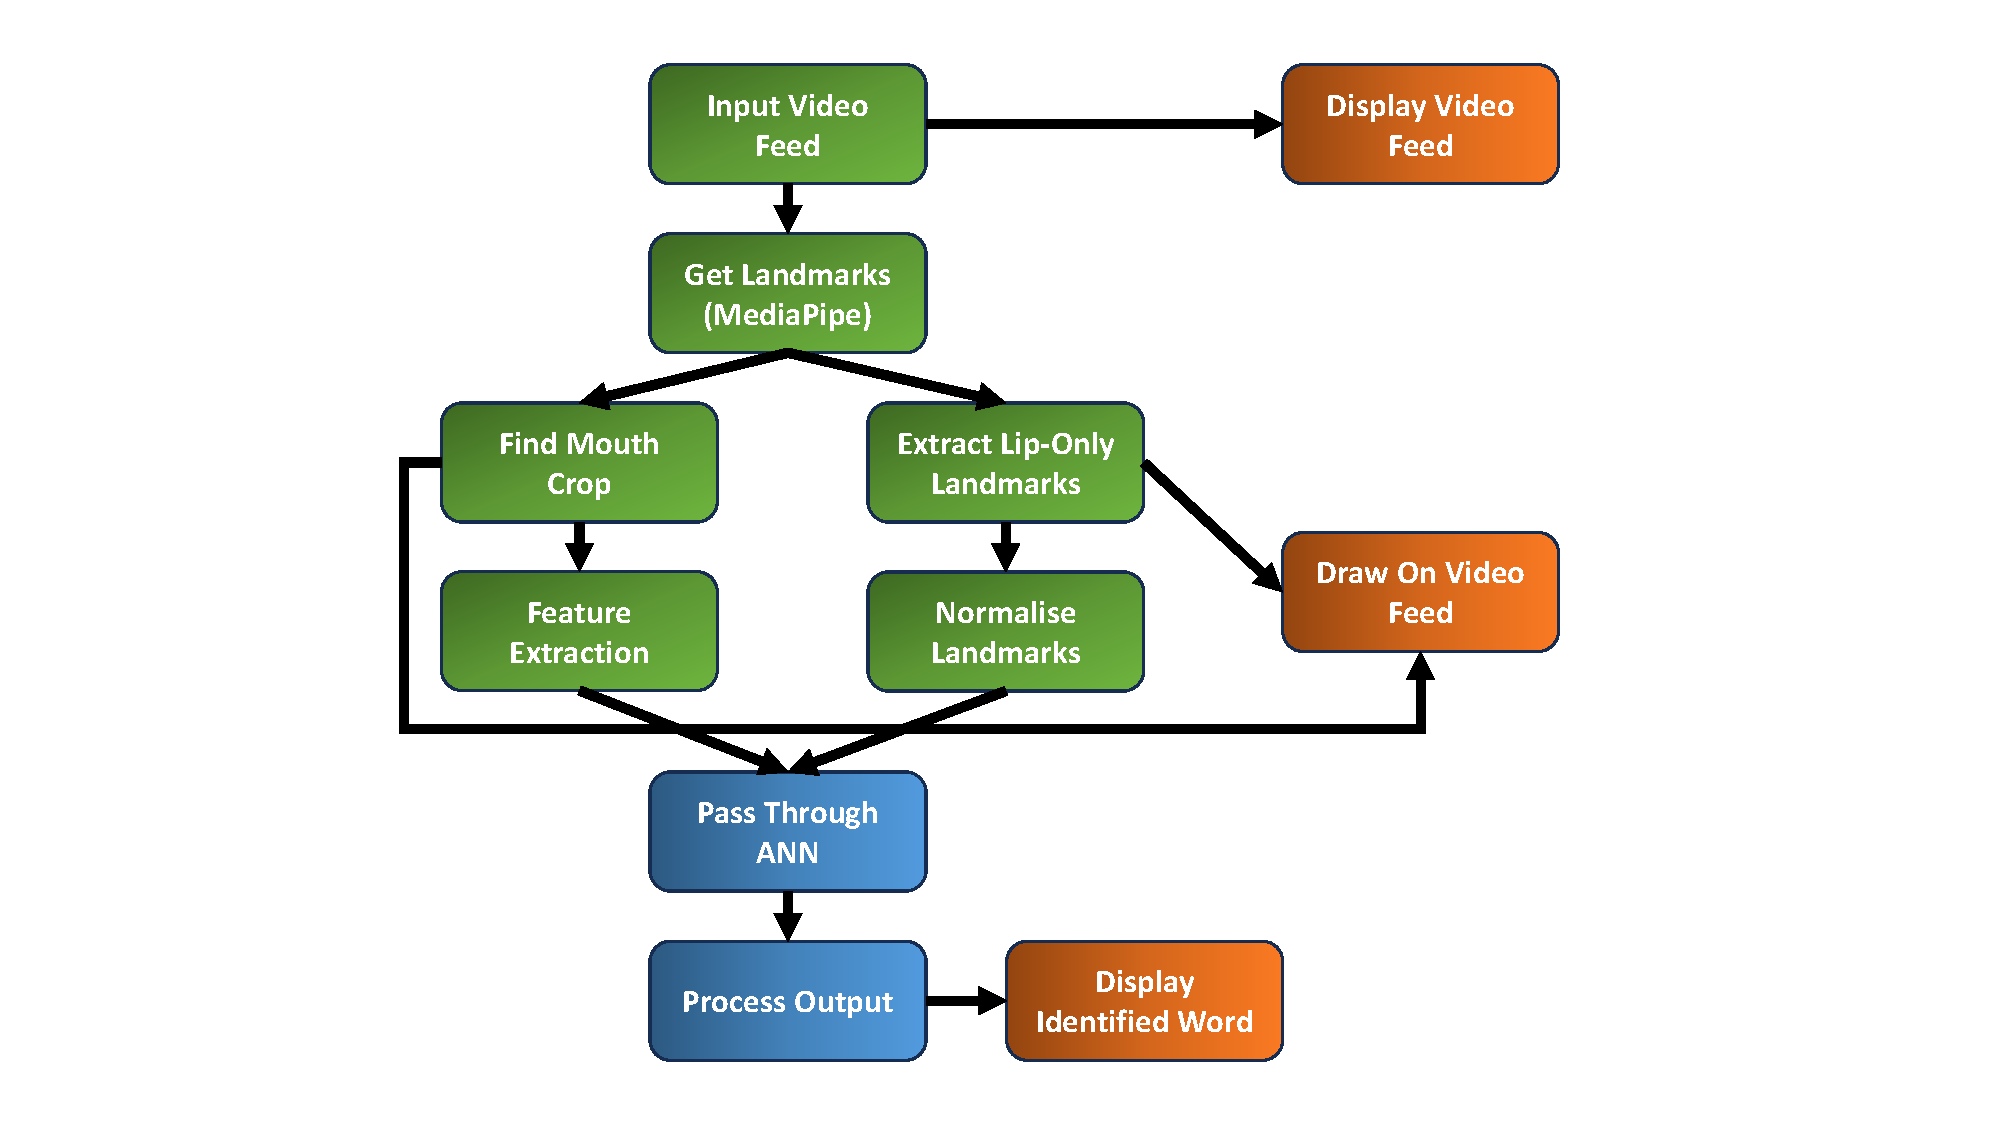
\includegraphics[width=1\textwidth]{GUI Workflow.pdf}
\caption[Inference workflow of the proposed lip reading \acrshort{gui}.]{Inference workflow of the proposed lip reading \acrshort{gui}. The \acrshort{gui} will have a constant video stream. It will detect people, extract data and pass it through the optimised model. The identified words will then be displayed on the screen. Green boxes represent stages required for data capture, blue for running the \acrshort{ann} and orange for displaying the results.}
\label{fig:gui diagram}
\end{figure}
Shown in Figure~\ref{fig:gui diagram}, the \acrshort{gui} was constructed with a specific workflow for capturing images, processing them and performing inference. The workflow was used to capture the required information to pass into the lip reading models outlined in Chapter~\ref{cha:results} and identify the words being spoken.\\
There are three main parts of this workflow
\begin{enumerate}
    \item Data capture
    \item Running the \acrlong{ann}
    \item Displaying the results
\end{enumerate}
For data capture a similar method was carried out as specified in Section~\ref{sec: Data Generation Pipeline}. MediaPipe was employed to identify faces, generate landmarks and produce visual and landmark features.\\
Running the \acrshort{ann} was a more configurable process, controlled by the \acrshort{gui}'s widgets. The visual and landmark data from data capture were passed into the \acrshort{ann} selected within the \acrshort{gui}.\\
The output of this was processed based on the selected model. The classes used were configured, as shown in Listing~\ref{lst: Model Mappings}, based on how the different models were trained. For models that were trained to classify data into whole words, the word-based dictionary was selected to translate model output.\\
\begin{lstlisting}[language=Python, caption={[The label mappings used for the different models.]{The label mappings used for the different models. This shows the mapping from the model output to the word labels for each different model output type.}}, label={lst: Model Mappings}]
word_based = {0: "ABOUT", 1: "BELIEVE", 2: "CHANCE", 3: "FAMILY"}
letter_based = {16: " ", 1: "A", 2: "B", 3: "C", 4: "E", 5: "F", 6: "H", 7: "I", 8: "L", 9: "M", 10: "N", 11: "O", 12: "T", 13: "U", 14: "V", 15: "Y",}
phoneme_based = {1: 'AE1', 2: 'AH0', 3: 'AW1', 4: 'B', 5: 'CH', 6: 'F', 7: 'IH0', 8: 'IY0', 9: 'IY1', 10: 'L', 11: 'M', 12: 'N', 13: 'S', 14: 'T', 15: 'V', 16: ' '}
viseme_based = {1: 'aa', 2: 'ah', 3: 'ch', 4: 'eh', 5: 'f', 6: 'iy', 7: 'k', 8: 'p', 9: 't', 10: 'uh', 11: ' '}
\end{lstlisting}
However, a major design decision came in the form of configuring the input to models. The correspondence of frames to labels for some models was many-to-one, whilst for others it was one-to-one. Therefore, in addition to the label translation, each model included the number of frames required for a single prediction. For the many-to-one models, a buffer of data (the ``frame buffer") was maintained for each frame ready to be passed through the model at the correct time. Only once the frame buffer was full was a prediction made before the buffer was emptied, ready for new frames to be accepted.\\
Displaying the results involved displaying the current view of the selected camera, displaying the landmarks or bounding box (according to user configuration) found using MediaPipe and displaying the processed output from the \acrshort{ann}.
\subsection{System Structure}
\begin{figure}
\centering
    \subfloat[\centering Mockup iteration 1]{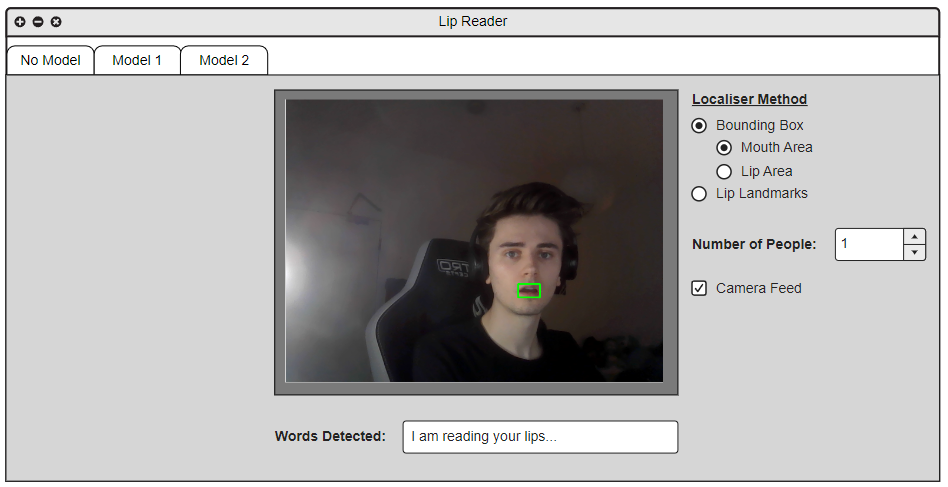
\includegraphics[width=0.5\textwidth]{GUI Mockup 1.png}}%
    % \qquad
    \subfloat[\centering Mockup iteration 2]{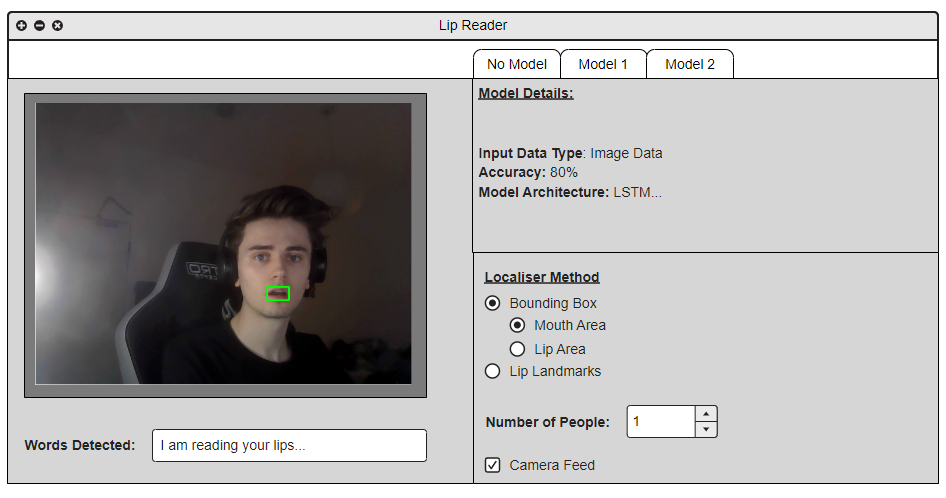
\includegraphics[width=0.5\textwidth]{GUI Mockup 2.png}}\\
    \subfloat[\centering Mockup iteration 3]{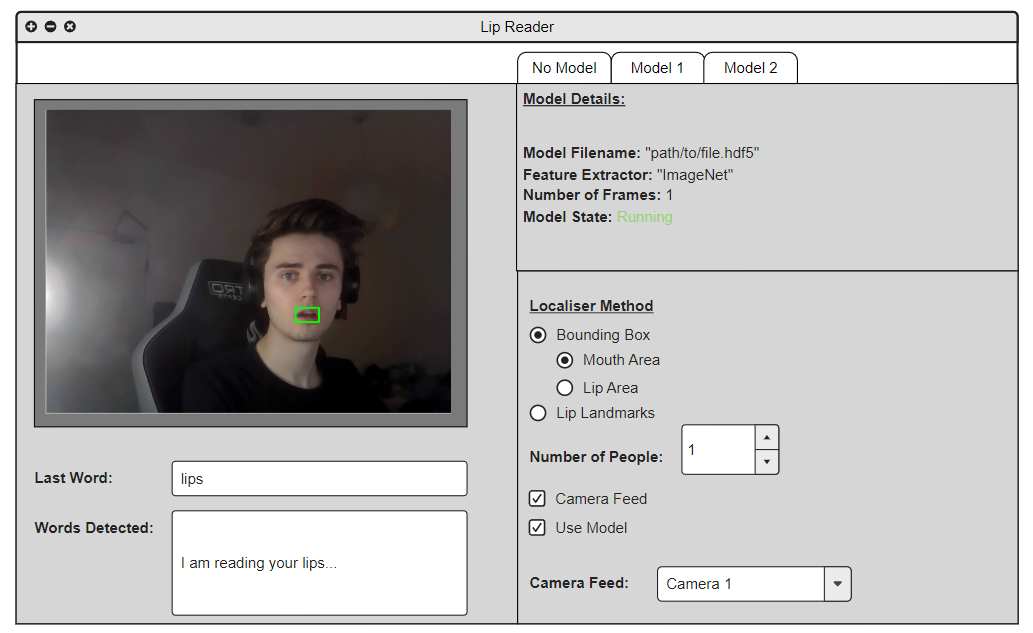
\includegraphics[width=0.5\textwidth]{GUI Mockup 3.png}}%
\caption[The three mockup iterations of the \acrfull{gui}]{The three mockup iterations of the \acrfull{gui}. The first stage included changing between models, realtime video feed and control over localisation. The second altered mainly the look of the system. The final mockup added further controls for the model, mainly in the inference methods, and more important model details.}
\label{fig:gui mockups}
\end{figure}
The design of the \acrshort{gui} went through three short iterations of mockups, as shown in Figure~\ref{fig:gui mockups}. All mockups were made using moqups\footnote{\url{https://moqups.com/}}. After these mockups were developed, the main \acrshort{gui} was produced using Tkinter. The remaining time within this project permitted the \acrshort{gui} to be extended, adding an extra tab within the window for model \gls{fine-tuning}. This is shown further in Figure~\ref{fig:annotated gui}.
\begin{figure}
\centering
    \subfloat[\centering Inference Tab]{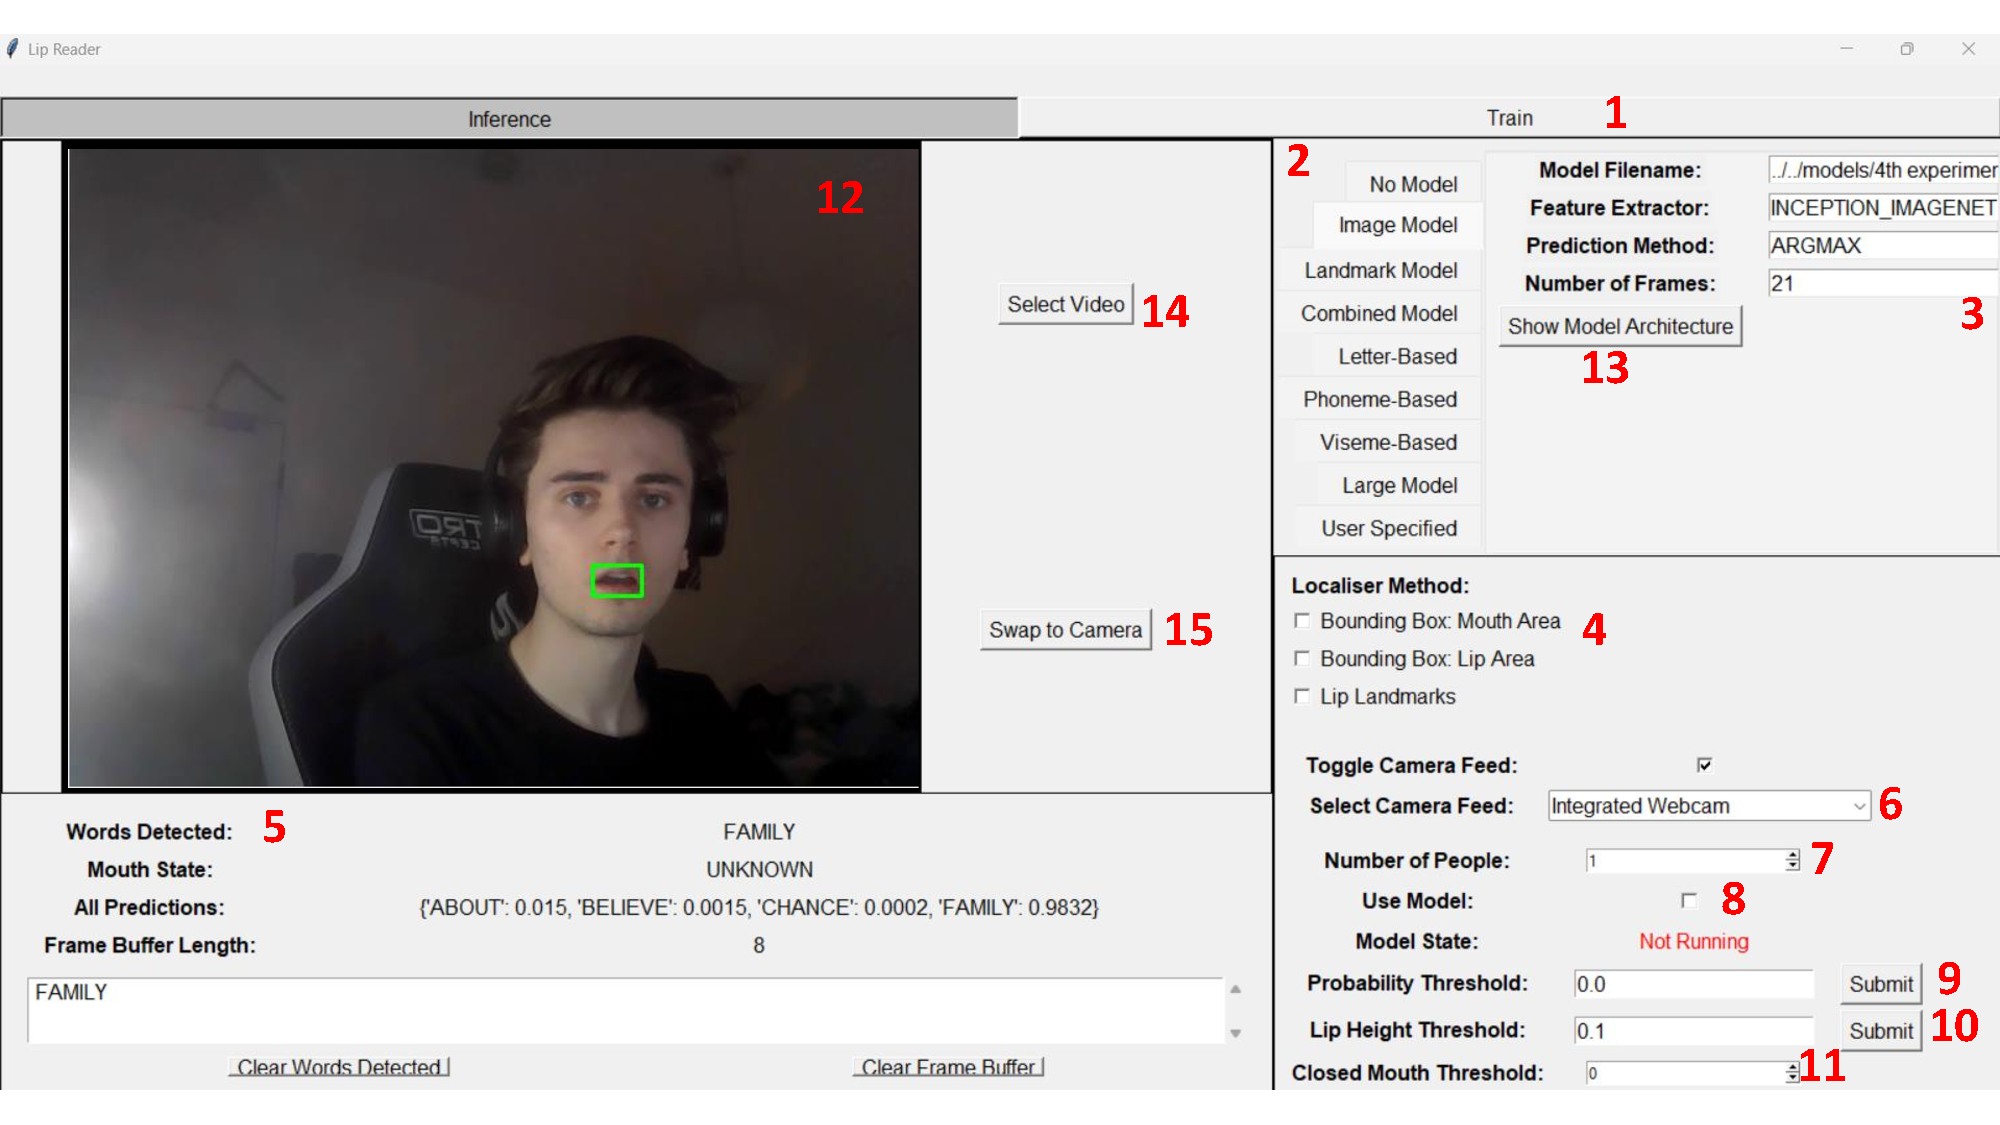
\includegraphics[width=0.5\textwidth]{Annotated GUI Inference.pdf}}
    \subfloat[\centering Training (\gls{fine-tuning}) Tab]{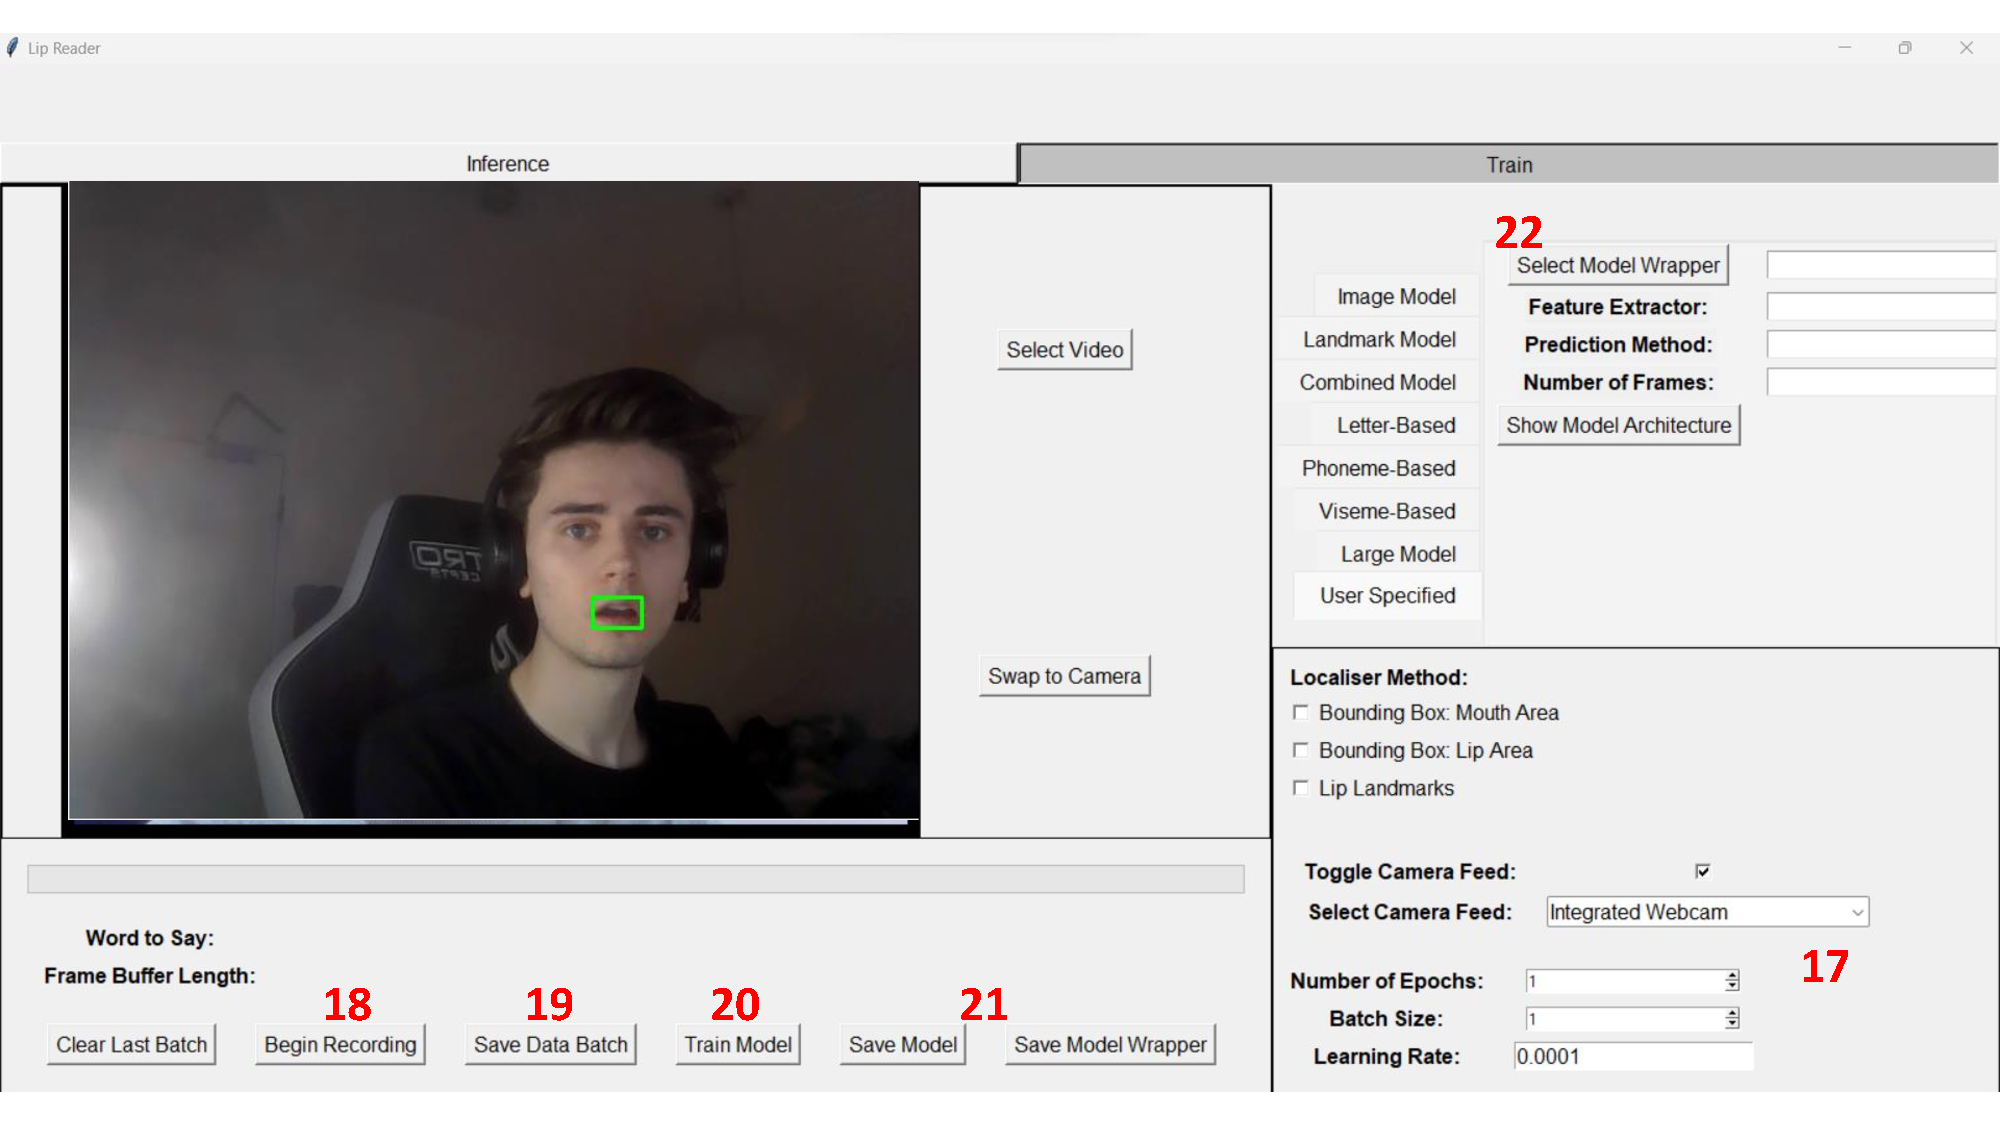
\includegraphics[width=0.5\textwidth]{Annotated GUI Train.pdf}}\\
\caption[The labelled \acrfull{gui}.]{The labelled \acrfull{gui}. This labels each of the primary features of the fully implemented \acrshort{gui}. Here both tabs for the \acrshort{gui} are shown: inference and training (or rather, \gls{fine-tuning}).}
\label{fig:annotated gui}
\end{figure}
The features of the \acrshort{gui} are presented below:
\begin{enumerate}
    \item \textbf{Mode Selector}: Used to change the interface between inference and training (or \gls{fine-tuning})
    \item \textbf{Model Selector}: Used to change between different trained models. Only a subset of the models are provided to select between. Note the change here that a vertical layout was employed rather than horizontal. This was to allow for better distinction between the different models
    \item \textbf{Model Properties}: This pane is used to give details about each of the different models
    \item \textbf{Localiser Method}: This configures display feed annotation, drawing bounding boxes around the lip or mouth area, or displaying the lip landmarks. This process is outlined more in Sections~\ref{sec: Visual Feature Extraction} and \ref{sec: Landmark Feature Extraction}
    \item \textbf{Prediction Frame}: This displays the current prediction, the past predictions and the frame buffer length (as it fills up). This displays the current mouth state (open or closed), the process for which is explained in Item~\ref{item: Lip Height Threshold} and Item~\ref{item: Closed Mouth Threshold}
    \item \textbf{Camera Feed Selection}: Python was used to detect all available cameras connected to the current device. These were then presented in a drop-down box for selection 
    \item \textbf{Number of People in Frame}: Used to configure MediaPipe to detect the correct number of people in the frame. Utilised to display bounding boxes for the lips of several people
    \item \textbf{Enable Model}: Used to begin running the model or pause it from making inference
    \item \textbf{Probability Threshold}: The threshold for prediction probabilities. Predictions below this predictions will be set to \textit{UNKNOWN}
    \item \textbf{Lip Height Threshold}: The threshold for the distance between the average of the upper landmarks and the average of the lower landmarks. Below this threshold the lips are considered to be together, and therefore closed, for the current frame \label{item: Lip Height Threshold}
    \item \textbf{Closed Mouth Threshold}: A threshold for the number of frames in a row that the mouth is closed for. If the number exceeds this value then predictions will stop being made as the lips are considered as being closed. This saves computation by having the model switch off for a person who isn't speaking. When set to 0 this feature is not used to stop predictions \label{item: Closed Mouth Threshold}
    \item \textbf{Display Area}: This displays the current feed of the selected camera
    \item \textbf{Model Architecture}: Clicking this button will open another window, displaying the model architecture of the currently selected model. This diagram is automatically generated in real-time using Keras util's plot\_model\footnote{\url{https://www.tensorflow.org/api_docs/python/tf/keras/utils/plot_model}} function
    \item \textbf{Select Video}: This creates a file dialogue box, allowing selection of a video file. This file will then be repeatedly played in the window and used for inference
    \item \textbf{Swap to Camera}: This swaps the feed back to the currently selected input stream
    \item \textbf{\Gls{fine-tuning} Configuration}: This area is used to modify and control the settings for model \gls{fine-tuning} such as the \acrshort{lr}, epochs and batch size \label{item: fine-tune settings}
    \item \textbf{Begin Recording}: Activates data collection, starting to collect frames from the input stream for the current word \label{item: begin recording} 
    \item \textbf{Save Data Batch}: This will temporarily save the data sample to be used for \gls{fine-tuning} later \label{item: save data} 
    \item \textbf{Train Model}: This model starts \gls{fine-tuning} of the model using the data \label{item: finetune} 
    \item \textbf{Model Saving}: These buttons are used to save the currently selected model or whole model wrapper to be loaded in and used through Item~\ref{item: load model}
    \item \textbf{Load Model}: Selecting the ``User Specified" model shows this feature. Clicking this button creates a dialogue, allowing a model wrapper file to be found and selected for use \label{item: load model} 
\end{enumerate}
One of the main, complex features of the \acrshort{gui} is that of stopping inference when the mouth is closed. This is controlled using Items~\ref{item: Closed Mouth Threshold} and \ref{item: Lip Height Threshold}. Item~\ref{item: Closed Mouth Threshold} controls the relative height between the upper and low lips. When this height is less than the threshold, the lips are considered closed. Item~\ref{item: Lip Height Threshold} controls inference associated with when the user has stopped speaking, stopping the model from predicting if it considers the speaker to have paused for a time.\\
Another feature worth further explanation is that of \gls{fine-tuning} lip reading models. To fine-tune the model, a user is presented with the classes of the currently selected model. They can select Item~\ref{item: begin recording} to begin recording data for \gls{fine-tuning} and Item~\ref{item: save data} to save that data internally. When Item~\ref{item: finetune} is selected \gls{fine-tuning} of the current model will begin. This will utilise the training settings configured within Item~\ref{item: fine-tune settings} to fine-tune the current model. This could take some time depending on the settings. The resulting model metrics will be printed to the interface and the user can then opt to save the new model using Item~\ref{item: save data}.